\documentclass[a4paper]{article}
\usepackage[english]{babel}
\usepackage[utf8]{vietnam}

%\usepackage{vntex}

%\usepackage[english,vietnam]{babel}
%\usepackage[utf8]{inputenc}

%\usepackage[utf8]{inputenc}
%\usepackage[francais]{babel}
\usepackage{a4wide,amssymb,epsfig,latexsym,multicol,array,hhline,fancyhdr}

\usepackage{amsmath}
\usepackage{lastpage}
\usepackage[lined,boxed,commentsnumbered]{algorithm2e}
\usepackage{enumerate}
\usepackage{color}
\usepackage{graphicx}		
\graphicspath{ {figures/} }
% Standard graphics package
\usepackage{listings}
\lstset{frame=tb,
  language=Python,
  aboveskip=3mm,
  belowskip=3mm,
  showstringspaces=false,
  columns=flexible,
  basicstyle={\small\ttfamily},
  numbers=none,
  numberstyle=\tiny\color{gray},
  keywordstyle=\color{blue},
  commentstyle=\color{dkgreen},
  stringstyle=\color{mauve},
  breaklines=true,
  breakatwhitespace=true,
  tabsize=3
}
\definecolor{dkgreen}{rgb}{0,0.6,0}
\definecolor{gray}{rgb}{0.5,0.5,0.5}
\definecolor{mauve}{rgb}{0.58,0,0.82}
\usepackage{array}
\usepackage{tabularx, caption}
\usepackage{multirow}
\usepackage{multicol}
\usepackage{rotating}
\usepackage{graphics}
\usepackage[a4paper,left=2cm,right=2cm,top=1.8cm,bottom=2.8cm]{geometry}
\usepackage{setspace}
\usepackage{epsfig}
\usepackage{tikz}
\usetikzlibrary{arrows,snakes,backgrounds}
\usepackage[bottom]{footmisc}
\usepackage[unicode]{hyperref}
\usepackage[labelformat=empty]{caption}

%can file puenc.def trong thu muc goc de option [unicode] tao ra bookmark bang tieng Viet
\hypersetup{urlcolor=blue,linkcolor=black,citecolor=black,colorlinks=true} 
%\usepackage{pstcol} 								
% PSTricks with the standard color package

\newtheorem{theorem}{{\bf Theorem}}
\newtheorem{property}{{\bf Property}}
\newtheorem{proposition}{{\bf Proposition}}
\newtheorem{corollary}[proposition]{{\bf Corollary}}
\newtheorem{lemma}[proposition]{{\bf Lemma}}


%\usepackage{fancyhdr}
\setlength{\headheight}{40pt}
\pagestyle{fancy}
\fancyhead{} % clear all header fields
\fancyhead[L]{
 \begin{tabular}{rl}
    \begin{picture}(25,15)(0,0)
    \put(0,-8){
\includegraphics[width=8mm, height=8mm]{hcmut.png}}
    %\put(0,-8){\epsfig{width=10mm,figure=hcmut.eps}}
   \end{picture}&
	%
\includegraphics[width=8mm, height=8mm]{hcmut.png} & %
	\begin{tabular}{l}
		\textbf{\bf \ttfamily Trường Đại học Bách Khoa - Đại học Quốc gia TP.HCM}\\
		\textbf{\bf \ttfamily Bộ môn Viễn Thông}
	\end{tabular} 	
 \end{tabular}
}
\fancyhead[R]{
	\begin{tabular}{l}
		\tiny \bf \\
		\tiny \bf 
	\end{tabular}  }
\fancyfoot{} % clear all footer fields
\fancyfoot[L]{\scriptsize \ttfamily Đồ án - Phục hồi màu cho ảnh xám, 05/2021}
\fancyfoot[R]{\scriptsize \ttfamily {\thepage /iv}}
\renewcommand{\headrulewidth}{0.3pt}
\renewcommand{\footrulewidth}{0.3pt}

%%%
\setcounter{secnumdepth}{4}
\setcounter{tocdepth}{3}
\makeatletter
\newcounter {subsubsubsection}[subsubsection]
\renewcommand\thesubsubsubsection{\thesubsubsection .\@alph\c@subsubsubsection}
\newcommand\subsubsubsection{\@startsection{subsubsubsection}{4}{\z@}%
                                     {-3.25ex\@plus -1ex \@minus -.2ex}%
                                     {1.5ex \@plus .2ex}%
                                     {\normalfont\normalsize\bfseries}}
\newcommand*\l@subsubsubsection{\@dottedtocline{3}{10.0em}{4.1em}}
\newcommand*{\subsubsubsectionmark}[1]{}
\makeatother

\begin{document}

\begin{titlepage}

\begin{center}
TRƯỜNG ĐẠI HỌC BÁCH KHOA - ĐẠI HỌC QUỐC GIA TP.HCM\\
BỘ MÔN VIỄN THÔNG
\end{center}

\vspace{1cm}

\begin{figure}[h!]
\begin{center}

\includegraphics[width=3cm]{hcmut.png}
\end{center}
\end{figure}

\vspace{1cm}


\begin{center}
\begin{tabular}{c}
\multicolumn{1}{l}{\textbf{{\Large TRÍ TUỆ NHÂN TẠO}}}\\
~~\\
\hline
\\
\multicolumn{1}{l}{\textbf{{\Large Đồ án}}}\\
\\
\textbf{\Huge Phục hồi màu cho ảnh xám}\\
\\
\hline
\end{tabular}
\end{center}

\vspace{3cm}

\begin{table}[h]
\begin{tabular}{rrl}

\hspace{2.7 cm} & GVHD: PGS.TS Hà Hoàng Kha & (hhkha@hcmut.edu.vn)\\
& Sinh viên: & Nguyễn Thành Trung - 1814515\\
\\\\\\\\\\

\end{tabular}
\end{table}

\begin{center}
{\footnotesize Hồ Chí Minh, 05/2021}
\end{center}
\end{titlepage}


%\thispagestyle{empty}
\pagenumbering{roman}
\newpage

\begin{center}
\huge
\textbf{Lời cảm ơn}
\end{center}

\indent
Em xin bày tỏ lòng biết ơn đến chân thành sâu sắc tới giáo viên hướng dẫn của em, thầy \textbf{PGS.TS Hà Hoàng Kha} - ``giảng viên bộ môn Viễn Thông'' đã trực tiếp giúp đỡ, hướng dẫn em hoàn thành đồ án này.\\

Dẫu vậy, do kiến thức chuyên ngành còn hạn chế nên trong quá trình nghiên cứu đề tài em vẫn còn nhiều thiếu sót khi tìm hiểu, đánh giá và trình bày về đề tài. Rất mong được sự quan tâm, góp ý của các thầy/cô giảng viên bộ môn để đề tài của em được đầy đủ và hoàn chỉnh hơn.\\


Em xin chân thành cảm ơn.\\\\\\

\hfill
\begin{tabular}{l@{}}
\textit{Tp. Hồ Chí Minh, ngày \textbf{04} tháng \textbf{05} năm \textbf{2021}.}\\\\
\hspace{3cm}\textbf{Sinh Viên}
\end{tabular}

\newpage

\begin{center}
\huge
\textbf{Tóm tắt đồ án}
\end{center}

\indent
Đồ án với mục tiêu nghiên cứu, tìm ra một mô hình có có khả năng tự động việc tô màu cho những ảnh xám, cũ đã mất màu để giúp cho quá trình phục chế màu được tiết kiệm thời gian. Đồ án được thực hiện nhờ vào việc áp dụng những kiến thức về \textbf{trí tuệ nhân tạo} (\textit{artificial intelligence}), cụ thể là \textbf{học sâu} (\textit{deep learning}).\\

Mô hình được xây dựng theo kiểu \textbf{mạng đối nghịch tạo sinh} (\textit{GAN - Generative Adversarial Network}) với Generator có kiến trúc Unet dựa theo mạng huấn luyện sẵn ResNet18, sau khi học đã có khả năng tự động tô màu những ảnh xám, cũ một cách chân thực, hợp lí.

\newpage

\tableofcontents

\newpage

% \thispagestyle{empty}
\renewcommand{\listfigurename}{Danh sách hình minh hoạ}
\listoffigures

\newpage

\pagenumbering{arabic}
\fancyfoot[R]{\scriptsize \ttfamily {\thepage}/\pageref{LastPage}}

%%%%%%%%%%%%%%%%%%%%%%%%%%%%%%%%%
\section{Giới thiệu}

\subsection{Tổng quát}
Nhu cầu phục chế ảnh màu từ ảnh xám không phải là hiếm. Thông thường là ảnh do tác động của thời gian, làm mất hoặc sai màu. Đôi khi lại là hình ảnh được chụp ở thời xưa, thời đại chưa có công nghệ chụp ảnh màu.\\
Hiện nay, hầu hết mọi người đều sử dụng phương pháp thủ công bằng tay. Tuy có sự giúp đỡ của các công cụ hỗ trợ chỉnh sửa hình ảnh, để có thể có một tấm ảnh đẹp cũng đòi hòi mất nhiều thời gian, có thể lên đến cả tháng đối với những bức ảnh có nhiều chi tiết.\\

\noindent
Thấy được những điều trên, em đã thử tìm kiếm các bài báo về cách thức có thể tự động phục chế màu cho ảnh bằng \textbf{máy học/học sâu} (\textit{Machine Learning/Deep Learning}).\footnote{Chi tiết trong phần \textbf{\nameref{references} tham khảo}} Từ đó xây dựng một mô hình tự động hoá việc tô màu.\\
Hầu hết ý tưởng cho mô hình của em tham khảo từ bài báo \href{https://arxiv.org/abs/1611.07004}{\textbf{Image-to-Image Translation with Condition Adversarial Networks}}, hay còn được biết với cái tên \textbf{pix2pix}, đưa ra giải pháp cho những vấn đề về image-to-image và một trong số đó có liên quan tới việc tô màu ảnh. 

\subsection{Mục tiêu}\label{objective}
Việc khôi phục màu cho ảnh đúng tuyệt đối như những gì được chụp là một chuyện gần như bất khả thi vì không ai có thể biết được thực sự màu của những đối tượng cần được tô màu một cách chắc chắn. Hơn thế nữa, việc một đối tượng có thể có nhiều màu phù hợp là chuyện rất đỗi bình thường. Ví dụ đơn giản như một quả chuối có thể màu lục khi chưa chín nhưng lại cũng có thể là màu vàng khi chín.

\begin{figure}[h!]
\centering
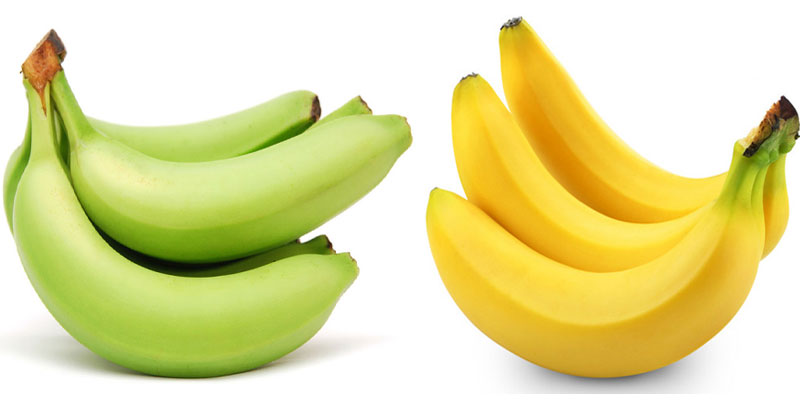
\includegraphics[width=15cm]{images/1_1.jpg}
\caption{Hình 1.1: Nải chuối có thể màu lục hoặc màu vàng. Nguồn: \href{https://bit.ly/3e7nqRs}{https://bit.ly/3e7nqRs}}
\end{figure}

\noindent
Nhưng không vì thế mà ta có thể tô bất cứ màu nào cho bất cứ vật thể nào, giả sử như việc tô màu da người là màu xanh biển hoặc mặt trời thì màu xanh lá, trông không được đúng đắn cho lắm.\\
Trên những cơ sở đó, mục tiêu của em khi lên kế hoạch tìm hiểu và thực hiện đề tài này là xây dựng được một mô hình có thể dự đoán màu của những đối tượng trong ảnh xám một cách hợp lí hơn là chính xác tuyệt đối. Chất lương dự đoán của mô hình cũng không mong đợi có thể bằng được so với làm thủ công, nhưng cũng tiết kiệm thời gian hơn rất nhiều.

%%%%%%%%%%%%%%%%%%%%%%%%%%%%%%%%%
\section{Xử lí bài toán}

\subsection{Lựa chọn không gian màu}

\subsubsection{Không gian màu RGB}
Hầu hết khi làm việc với ảnh số, ta hay làm việc với ảnh \textbf{RGB}, tức ảnh có 3 kênh màu đỏ-lục-lam (\textit{red-green-blue}). Mỗi điểm ảnh (\textit{pixel}) sẽ có 3 giá trị \textbf{R-G-B}, mỗi giá nằm trong đoạn $[0, 255]$, tương ứng với 3 kênh màu để tạo nên được màu của chính điểm ảnh.

\begin{figure}[h!]
\centering
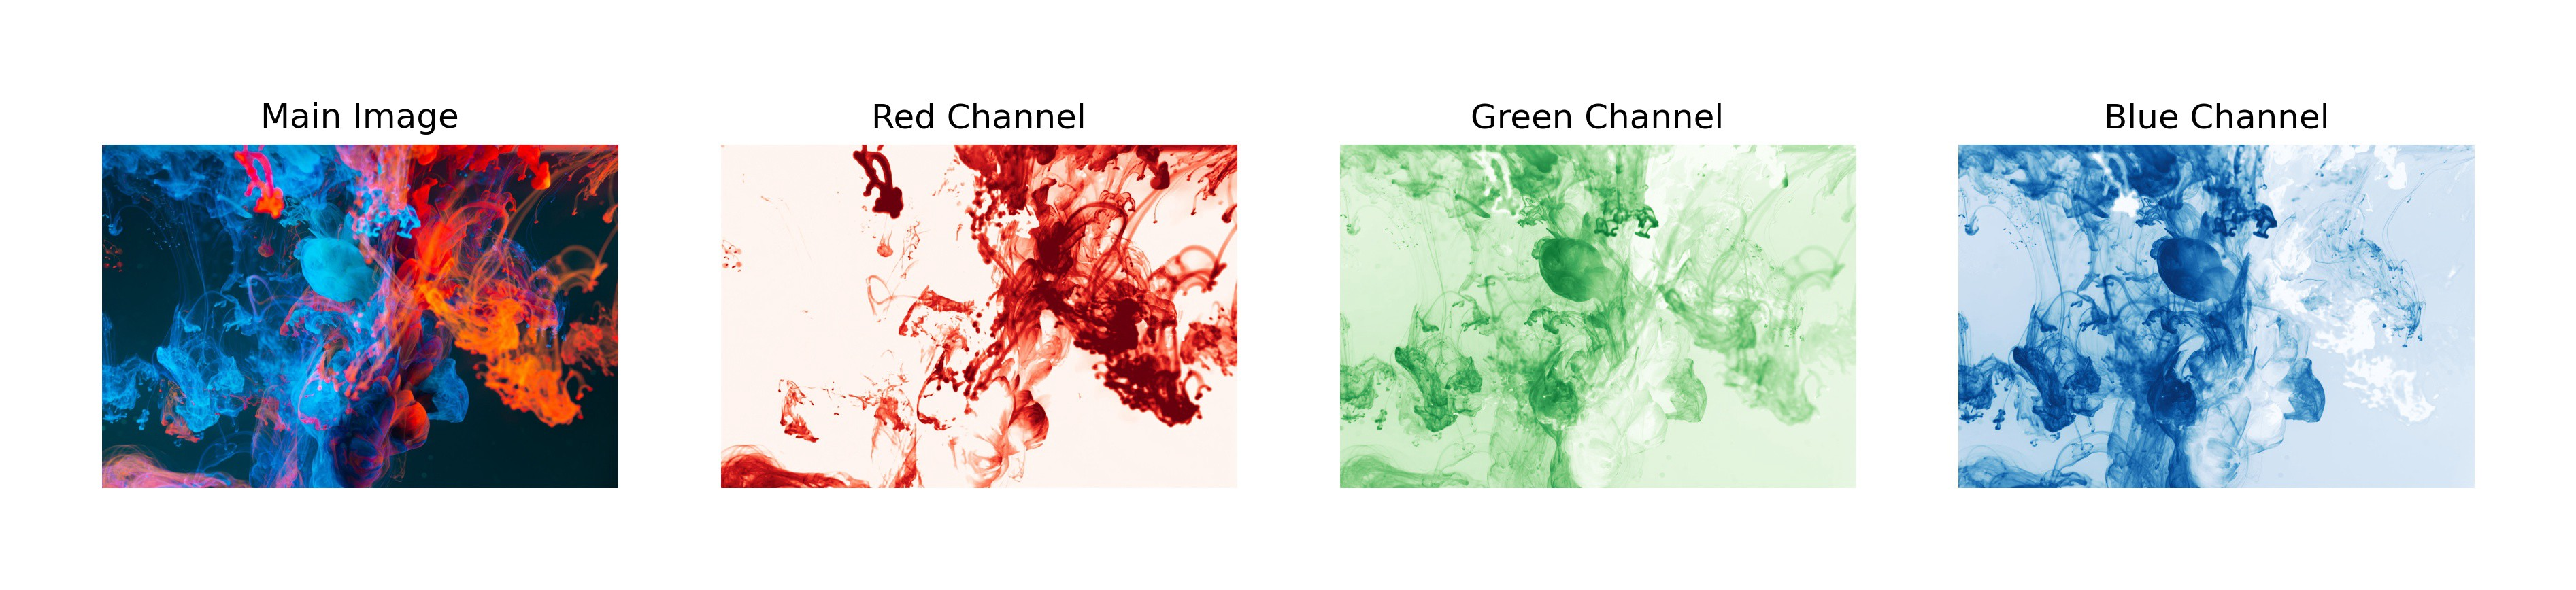
\includegraphics[width=16.1cm]{images/2_1.jpeg}
\caption{Hình 2.1: Các kênh màu đỏ, lục và lam được tách ra riêng biệt. Nguồn: \href{https://bit.ly/3eKaaBj}{https://bit.ly/3eKaaBj}}
\end{figure}

\subsubsection{Không gian màu Lab}
Ngoài RGB, một không gian màu khác cũng được sử dụng nhiều là không gian màu \textbf{Lab}, không gian này cũng quan tấm đến 3 thông số của mỗi điểm ảnh. Thông số đầu tiên là \textbf{L} (\textit{Lightness}) đại diện cho độ sáng của của mỗi điểm ảnh. 2 thông số còn lại là \textbf{a} và \textbf{b} sẽ mang thông tin lần lượt là lục-đỏ (\textit{green-red}) và vàng-lam (\textit{yellow-blue}). Giá trị \textbf{a} càng thấp thì lục nhiều, đỏ ít. Ngược lại thì lục ít, đỏ nhiều và tương tự với giá trị \textbf{b}.

\begin{figure}[h!]
\centering
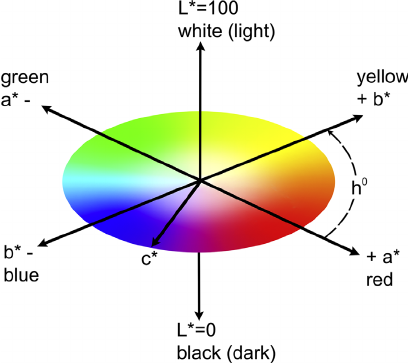
\includegraphics[width=5.8cm]{images/2_2.png}
\caption{Hình 2.2: Không gian màu Lab. Nguồn: \href{https://bit.ly/3nFIQIp}{https://bit.ly/3nFIQIp}}
\end{figure}

\noindent
Với giá trị \textbf{L}, giá trị sẽ nằm trong đoạn $[0, 100]$. Riêng 2 giá trị còn lại, không có cụ thể một khoảng nhất định, mà tuỳ thuộc vào phần mềm, chương trình mà ta sử dụng. Thường sẽ là đoạn $[-128, 127]$, tuy nhiên mô hình của em không sử dụng khoảng giá trị trên. Chi tiết về vấn đề này em sẽ làm rõ ở phần \textbf{3.3 \nameref{normalization}}.

\begin{figure}[h!]
\centering
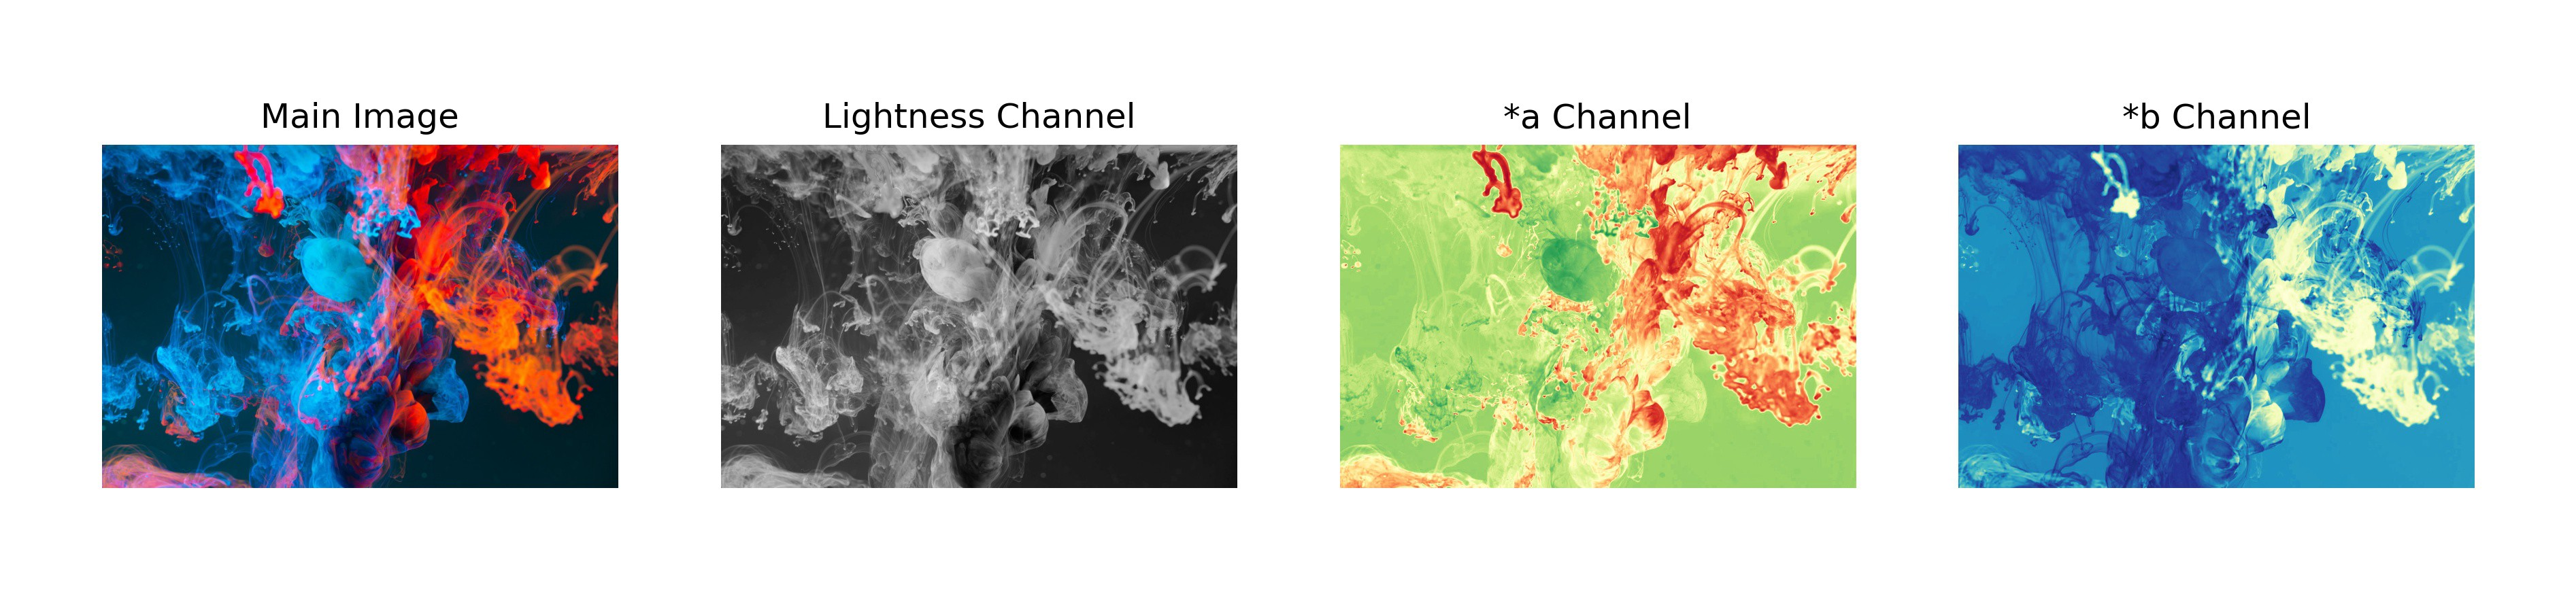
\includegraphics[width=16.1cm]{images/2_3.jpeg}
\caption{Hình 2.3: Các giá trị \textbf{L}, \textbf{a} và \textbf{b} được tách ra riêng biệt. Nguồn: \href{https://bit.ly/3eKaaBj}{https://bit.ly/3eKaaBj}}
\end{figure}

\subsubsection{Lựa chọn Lab thay vì RGB}
Khi tìm hiểu hầu hết các bài báo, em nhận thấy rằng hầu như không ai sử dụng không gian màu RGB để xử lí bài toán này mà thay vào đó là sử dụng Lab. Tuy lí do không được đề cập cụ thể trong các bài báo, em có thể đưa ra một số lí do để giải thích cho việc này.\\
Khi ta sử dụng không gian màu Lab, ta có thể tận dụng thông số \textbf{L} tức chỉ độ sáng (mức xám) và dự đoán 2 thông số còn lại. Không gian ta cần phải quan tâm có xấp xỉ $256^2 = 65,536$ khả năng. Khi đó, kết quả cuối cùng của ta chính là việc kết hợp đầu vào \textbf{L} và thông số \textbf{a}, \textbf{b} dự đoán được.\\ Trong khi đó, nếu sử dụng RGB, mô hình của chúng ta sẽ cần phải dự đoán tới 3 thông số là \textbf{R}, \textbf{G} và \textbf{B}. Điều này dẫn đến không gian kết quả của ta lên đến $256^3 = 16,777,216$ khả năng.\\
Chênh lệch khoảng hơn 16 triệu khả năng. Như vậy, mô hình cần phải phức tạp hơn, khó để có thể xây dựng cũng như huấn luyện. Vì vậy, việc lựa chọn không gian màu Lab không chỉ không giảm chất lượng màu mà còn giúp bài toán của chúng ta dễ dàng xử lí hơn.

\subsection{Một số phương pháp đơn giản}

\subsubsection{Đánh dấu màu vài điểm ảnh và dùng thuật toán lan}
Từ một tấm ảnh xám đầu vào, ta sẽ vẽ một vài màu cơ bản từ đó làm nền tảng, định hướng cho mô hình. Ý tưởng này xuất phát từ quan sát rằng, những điểm ảnh có độ sáng gần bằng nhau (mức xám xấp xỉ) và có khoảng cách trên ảnh gần nhau sẽ có khả năng tương tự cao dẫn đến màu giống nhau.

\begin{figure}[h!]
\centering
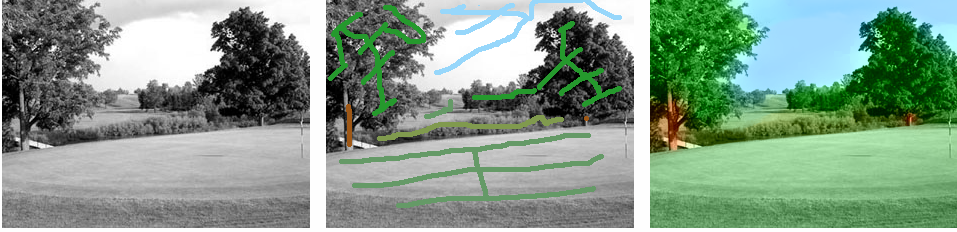
\includegraphics[width=15cm]{images/2_4.png}
\caption{Hình 2.4: Mô tả ý tưởng thuật toán. Nguồn: \href{https://bit.ly/3eKdmwN}{https://bit.ly/3eKdmwN}}
\end{figure}

\subsubsection{Dựa vào màu của ảnh có bố cục tương tự}
Ý tưởng thuật toán khá giống các bài toán phân loại (\textit{classification}), ta sẽ chọn ra một tấm ảnh có bố cục tương tự rồi dựa vào màu của ảnh đó kết hợp chỉnh sửa để đưa ra dự đoán.

\begin{figure}[h!]
\centering
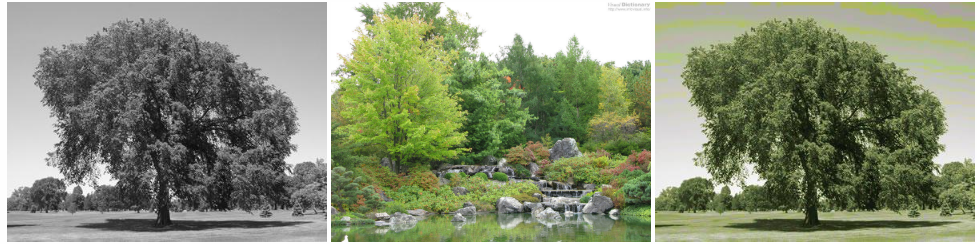
\includegraphics[width=15cm]{images/2_5.png}
\caption{Hình 2.5: Mô tả ý tưởng thuật toán. Nguồn: \href{https://bit.ly/3eKdmwN}{https://bit.ly/3eKdmwN}}
\end{figure}

\noindent
Vì chưa thực sự tìm hiểu sâu về hai phương pháp trên, nên em xin phép không đi sâu vào phần cách thức thuật toán hoạt động.

\subsubsection{Hạn chế}
Cả hai phương pháp còn khá là thủ công, chưa tự động được khi ta phải vẽ màu định hướng hoặc là chọn ảnh có bố cục tương tự.\\
Với phương pháp \textbf{Đánh dấu màu vài điểm ảnh và dùng thuật toán lan} sẽ gặp khó khăn khi bức ảnh có nhiều chi tiết khác màu nhau thì sẽ gây nhiều khó khăn trong việc vẽ màu định hướng.\\
Việc tìm bố cục tương tự với bức ảnh đầu vào cũng là một bài toán không hề đơn giản, điều này khiến phương pháp \textbf{Dựa vào màu của ảnh có bố cục tương tự} trở nên bất khả thi khi chưa tìm được ảnh có bố cục tương tự ưng ý.

\subsection{Phương pháp sử dụng Mạng đối nghịch tạo sinh (GAN - Generative Adversarial Network) kết hợp mô hình mạng Unet}

Đây là phương pháp mà em đã chọn để xử lí cho bài toán này, để có thể hiểu được kiến trúc mô hình mạng này, ta sẽ xem xét những thành phần cơ bản của mô hình. Tuy vậy, sẽ không đi sâu mà chỉ giới thiệu.

\subsubsection{Mạng đối nghịch tạo sinh - GAN}
Mạng GAN thuộc nhóm mô hình sinh dữ liệu mới. Dữ liệu sinh ra nhìn như thật nhưng không phải thật. Ví dụ như ảnh mặt người dưới đây là do GAN sinh ra, không phải mặt người thật.

\begin{figure}[h!]
\centering
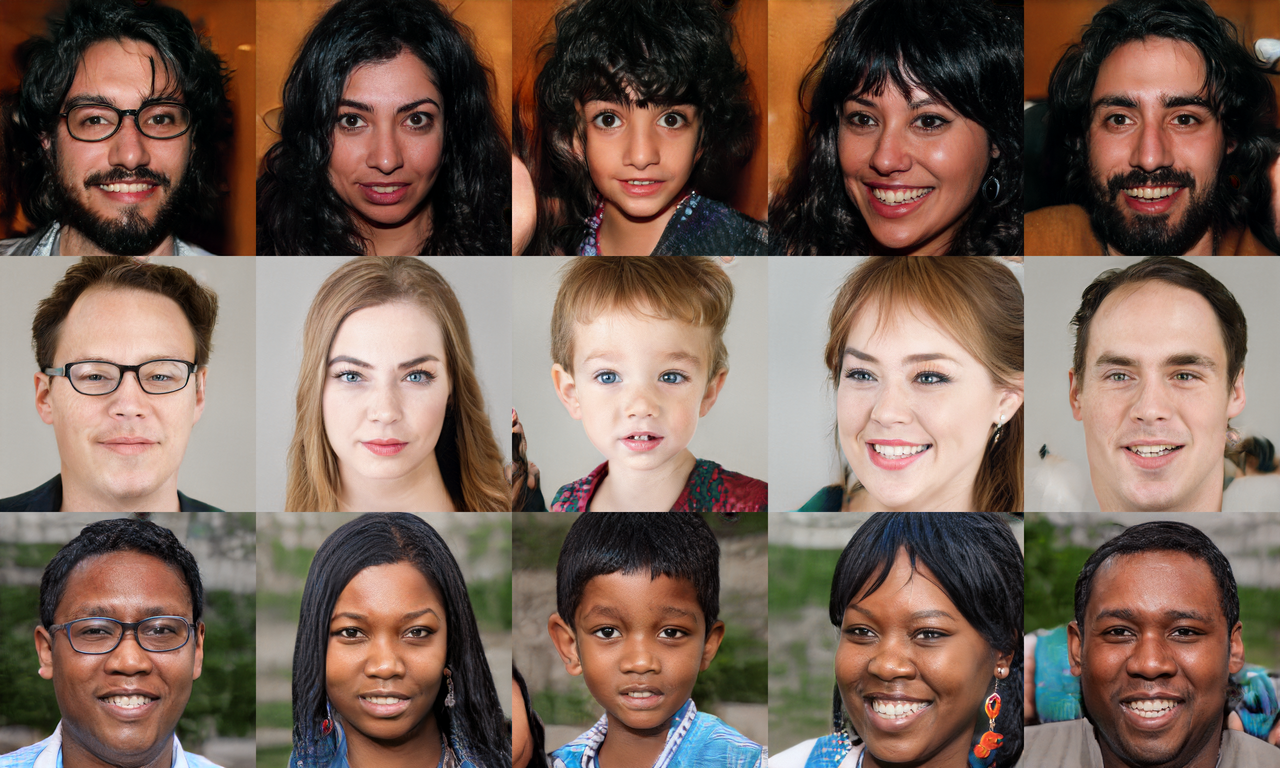
\includegraphics[width=13cm]{images/2_6.PNG}
\caption{Hình 2.6: Ảnh mặt người sinh ra bởi StyleGAN. Nguồn: \href{https://github.com/NVlabs/stylegan}{https://github.com/NVlabs/stylegan}}
\end{figure}

\noindent
G - Generative ý chỉ sinh, N - Network là mạng, còn A - Adversarial là đối nghịch. Lí do là trong mạng này được tạo nên từ sự kết hợp giữa 2 mạng là G - Generator và D - Discriminator, luôn luôn đối nghịch nhau trong quá trình huấn luyện.\\
Trong khi Generator cố gắng sinh ra các dữ liệu giống như thật thì Discriminator cố gắng phân biệt đâu là dữ liệu được sinh ra từ Generator và đâu là dữ liệu thật.\\

\noindent
Giả sử như bài toán đưa cho GAN là sinh ra tiền giả giống như tiền thật để có thể dùng được, Generator là người làm tiền giả, còn Discriminator giống như cảnh sát. Người làm tiền giả sẽ cố gắng làm ra những tờ tiền giả làm sao để cảnh sát không biết đó là giả, còn cảnh sát thì cố gắng học để phân biệt được tiền nào là giả, tiền nào là thật.\\
Mục tiêu cuối cùng của GAN là người làm tiền giả phải có khả năng làm tiền giả sao cho cảnh sát không phân biệt được đâu là thật đâu là giả (50/50) để đem tiền giả đi tiêu thụ.\\
Trong quá trình huấn luyện mạng GAN thì nhiệm vụ của cảnh sát là học cách phân biệt tiền giả và tiền thật, bên cạnh đó là nói cho người làm tiền giả là nên làm giả như thế nào cho tốt hơn. Dần dần thì người làm tiền giả sẽ làm ra được tiền giống tiền thật và cảnh sát cũng trở nên thành thạo trong việc phân biệt tiền thật hay giả.\\

\noindent
Ý tưởng của GAN bắt nguồn từ \href{https://cs.stanford.edu/people/eroberts/courses/soco/projects/1998-99/game-theory/nonzero.html}{Non-Zero-Sum Games}\footnote{Stanford, \lq Non-Zero-Sum Games\rq, \href{https://stanford.io/3nCiLKq}{https://stanford.io/3nCiLKq}}, là một trò chơi đối kháng giữa 2 người, nếu một trong hai người thắng, thì người còn lại sẽ thua. Ở mỗi lười, thì cả 2 đều muốn tối đa hoá cơ hội thắng của mình và tối thiểu hoá cơ hội thắng của đối phương. Trong lý thuyết trò chơi thì mô hình sẽ hội tụ khi cả Generator và Discriminator đạt tới trạng thái cân bằng Nash (\textit{Nash equilibrium}\footnote{Jørgen Veisdal, \lq The Nash equilibrium, explained\rq, \href{https://bit.ly/3ea57Lr}{https://bit.ly/3ea57Lr}}), tức là các bước tiếp theo của bất cứ ai trong hai người đều không làm thay đổi cơ hội thẳng của ai cả.

\begin{figure}[h!]
\centering
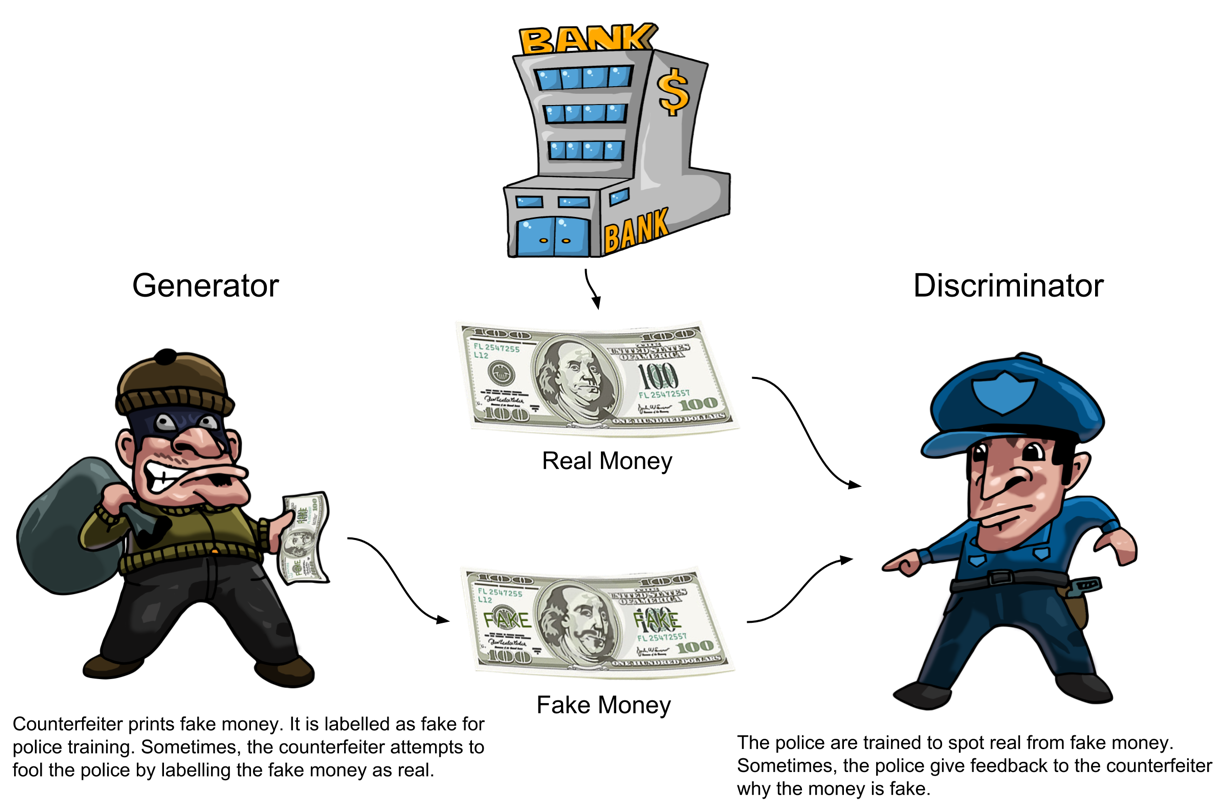
\includegraphics[width=9.5cm]{images/2_7.png}
\caption{Hình 2.7: Minh hoạ Generator và Discriminator trong mạng GAN. Nguồn: \href{https://bit.ly/3ue1M3r}{https://bit.ly/3ue1M3r}}
\end{figure}

\subsubsection{Mô hình mạng Unet}
Unet là một kiến trúc được phát triển nhằm phân vùng các cấu trúc nơ-ron thần kinh trong não người. Kiến trúc này lần đầu được áp dụng đã giành chiến thắng trong cuộc thi EM segmentation challenge at ISBI 2012.\footnote{ISBS Challenge: Segmentation of neuonal structures in EM stacks, \href{http://brainiac2.mit.edu/isbi\_challenge/home}{http://brainiac2.mit.edu/isbi\_challenge/home}}

\noindent
Mạng Unet bao gồm 2 nhánh đối xứng nhau hình chữ U nên được gọi là Unet. Kiến trúc mạng bao gồm 2 phần là \textbf{thu hẹp} (\textit{contraction}) ở nhánh trái và \textbf{phần mở rộng} (\textit{expansion}) ở nhánh phải. Mỗi phần sẽ thực hiện một nhiệm vụ riêng như sau:

\begin{itemize}
    \item Phần thu hẹp: làm nhiệm vụ trích lọc đăc trưng để tìm ra bối cảnh của hình ảnh (\textit{WHAT}). Vai trò của phần thu hẹp tương tự như một Encoder. Một mạng Deep CNN sẽ đóng vai trò trích lọc đặc trưng. Lý do nhánh được gọi là thu hẹp vì kích thước dài và rộng của các tầng giảm dần, hiểu nôm na là giảm độ phân giải (\textit{resolution}).
    
    \item Phần mở rộng: Gồm các tầng đối xứng tương ứng với các tầng của nhánh thu hẹp. Quá trình làm tăng kích thước tầng gọi là Upsampling, hiểu theo một cách đơn giản là hàm ngược của tích chập (\textit{Deconvolution}) để tăng lại độ phân giải của ảnh đề biết được vị trí (\textit{WHERE}) từ đó đánh dấu nhãn của từng điểm ảnh.
\end{itemize}

\noindent
Đặc trưng riêng trong cấu trúc của Unet đó là áp dụng kết nối tắt đối xứng giữa các tầng của nhánh bên trái tương ứng với các tầng bên nhánh bên phải.
\begin{figure}[h!]
\centering
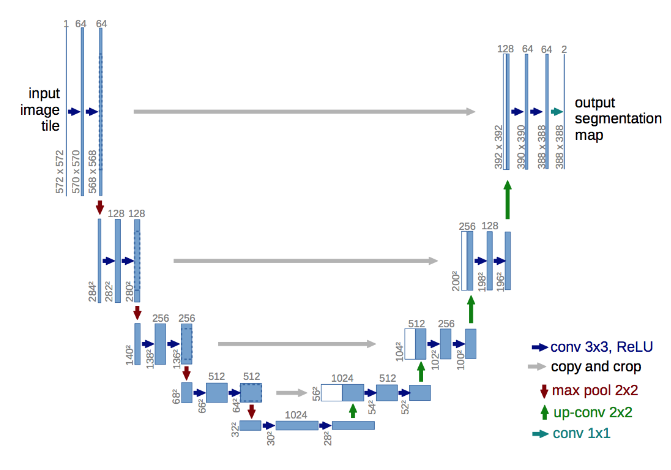
\includegraphics[width=9.5cm]{images/2_8.png}
\caption{Hình 2.8: Kiến trúc mô hình mạng Unet. Nguồn: \href{https://arxiv.org/abs/1505.04597}{https://arxiv.org/abs/1505.04597}}
\end{figure}

\noindent
Mô hình mạng Unet này sẽ được áp dụng vào Generator trong mô hình mạng GAN. Hay nói cách khác, ta sẽ dùng mạng Unet để làm Generator.

\subsection{Kiến trúc mô hình chính}
Với bài toán tô màu thì mục tiêu là từ đầu vào \textbf{L} (độ sáng - mức xám) của từng điểm ảnh ta sẽ dự đoán được cặp \textbf{(a, b)} để kết hợp tạo nên một tấm trong không gian màu Lab. Công việc này sẽ được G - Generator đảm nhận\\
Như vậy, để D - Discriminator phân biệt được đâu là thật giả, ta cần phải đưa vào cho Discriminator cả đầu vào lẫn đầu ra. Đây chính là điều kiện xác suất cho dự đoán của Discriminator và cũng chính là điểm khác biệt so với GAN thông thường, khi Discriminator được nhìn thấy dữ liệu đầu vào thay vì chỉ mỗi Generator.

\begin{figure}[h!]
\centering
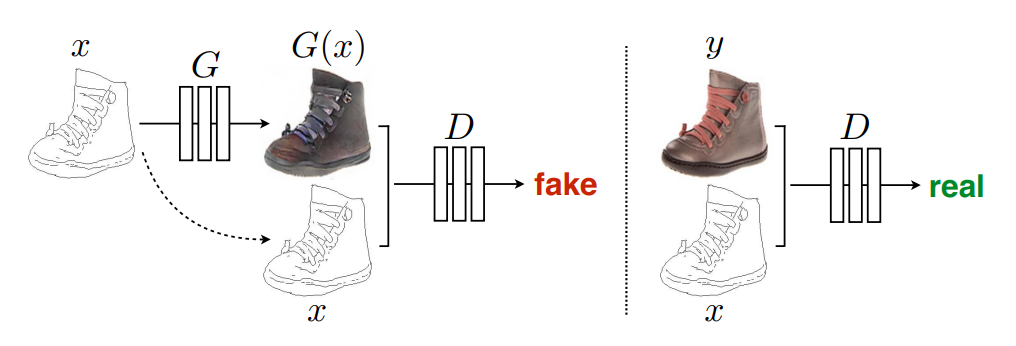
\includegraphics[width=13cm]{images/2_9.PNG}
\caption{Hình 2.9: Mô hình GAN dự đoán ảnh dựa vào đường viền. Nguồn: \href{https://arxiv.org/abs/1611.07004}{https://arxiv.org/abs/1611.07004}}
\end{figure}

\noindent
Do đó, hàm mất mát của mô hình GAN chúng ta cũng sẽ khác biệt một chút so với một mạng GAN thông thường, cụ thể là:
\begin{align*}
    \mathcal{L}_{cGAN}(G, D) = \mathbb{E}_{x, y}\left[\log D\left(x, y\right)\right] + \mathbb{E}_{x, z}\left[\log \left(1 - D\left(x, G\left(x, z\right)\right)\right)\right]
\end{align*}

\noindent
Trong đó, $x$ là đầu vào, chính là \textbf{L}, còn $y$ đầu ra là \textbf{(a, b)}. Còn $z$ là nhiễu (\textit{noise}) tạo ra từ việc \textbf{bỏ học} (\textit{dropout}).\footnote{Cụ thể được đề cập trong bài báo ``\textbf{Image-to-Image Translation with Conditional Adversarial Networks}'' là ``Instead, for our final models, we provide noiseonly in the form of dropout, applied on several layers of ourgenerator at both training and test time.''}\\
Nếu ta không dùng kỹ thuật bỏ học, mô hình vẫn sẽ có thể được huấn luyện và đưa ra kết quả dự đoán tốt tuy nhiên không được tổng quát, tức kết quả dự đoán của mô hình sẽ khá bị bó buộc khi phân phối sẽ chỉ có thể là hàm delta.\footnote{Cụ thể được đề cập trong bài báo ``\textbf{Image-to-Image Translation with Conditional Adversarial Networks}'' là ``Without $z$, the net could still learn a mapping from $x$ to $y$, but would produce deterministic outputs, and therefore fail to match any distribution other than a delta function.''}

\noindent
Một điểm khác biệt của Discriminator so với những Discriminator thông thường là Discriminator của chúng ta đúng hơn là Patch Discriminator. Lí do là thay vì chỉ trả về là một đầu ra là một số vô hướng (\textit{scalar}) thì Patch Discriminator của chúng ta sẽ phân loại từng vùng $N \times N$ của tấm ảnh là thật hay giả hay vì toàn bộ một lúc.\\

\noindent
GAN sẽ làm nhiệm vụ giúp cho màu chúng ta dự đoán được đẹp, giống như thật. Tuy nhiên không chỉ dừng lại đó, để có thể kiểm soát được chuyện mô hình tô màu được đẹp và giống thật, ta sẽ kết hợp với hàm mất mát dùng chuẩn 1 (\textit{norm 1} - L1 - \textit{mean absolute error}):
\begin{align*}
    \mathcal{L}_{L1}(G) = \mathbb{E}_{x, y, z}\left[\left|\left|y - G(x, z)\right|\right|_1\right]
\end{align*}
Tại sao lại là chuẩn 1 thay vì chuẩn 2 (chuẩn Euclid)? Lí do là chuẩn 2 có thường ``trừng phạt'' mất mát nhiều hơn so với chuẩn 1, do đó điều này làm bó buộc kết quả dự đoán của mô hình Generator làm cho mô hình có xu thể bảo thủ, sẽ dự đoán bằng cách lấy giá trị trung bình. Thay vì vậy, chuẩn 1 lại làm mềm việc ``trừng phạt'' này lại, khiến cho mô hình có thể đưa ra dự đoán ``phiêu lưu'' hơn. \\
Cuối cùng, mô hình ta cần phải tối ưu là:
\begin{align*}
    G^* = \arg\underset{G}{\min}\underset{D}{\max}\mathcal{L}_{cGAN}(G, D) + \lambda \mathcal{L}_{L1}(G)
\end{align*}
Trong đó, $\lambda$ là hệ số cân bằng để giúp cho sự chênh lệch giữa hai hàm mất mát không bị áp đảo nghiêng về một bên, khiến một hàm bị lu mờ trong quá trình huấn luyện.\\
Thông thường giá trị hàm mất mát của GAN sẽ có giá trị lớn hơn nhiều so với hàm chuẩn 1. Nên xu hướng chọn $\lambda$ sẽ là một số khá lớn, thông thường là $\lambda = 100$.

%%%%%%%%%%%%%%%%%%%%%%%%%%%%%%%%%
\section{Triển khai mô hình}

\subsection{Ngôn ngữ lập trình \& Thư viện chính}
Em sử dụng ngôn ngữ \textbf{Python} với sự hỗ trợ chính của thư viện \textbf{PyTorch}. Để cài đặt những công cụ này, có thể theo đường dẫn bên dưới:
\begin{itemize}
    \item Python: \href{https://www.python.org/downloads/}{https://www.python.org/downloads/}
    \item PyTorch \href{https://pytorch.org/get-started/locally/}{https://pytorch.org/get-started/locally/}
\end{itemize}
Bên cạnh đó, em cũng sử dụng thêm thư viện \textbf{fastai} (bản mới nhất). Để cài đặt, ta sử dụng lệnh sau trong môi trường Python:
\begin{lstlisting}
pip install fastai --upgrade
\end{lstlisting}

\noindent
Toàn bộ mã nguồn, cũng như những tệp liên quan trong quá trình hoàn thành mô hình có thể tìm thấy tại:
\begin{itemize}
    \item Github: \href{https://github.com/dee-ex/EE3151\_SEM202\_PROJECT}{https://github.com/dee-ex/EE3151\_SEM202\_PROJECT}
\end{itemize}

\subsection{Tập dữ liệu}
Tập dữ liệu được em chọn sử dụng là tập \href{https://cocodataset.org/#download}{\textbf{COCO}} có trong thư viện \textbf{fastai}, ta có thể dễ dàng tải về. Em quyết định chọn $10,000$ ảnh để huấn luyện, còn quá trình xác thực sẽ là $2,000$.

\begin{figure}[h!]
\centering
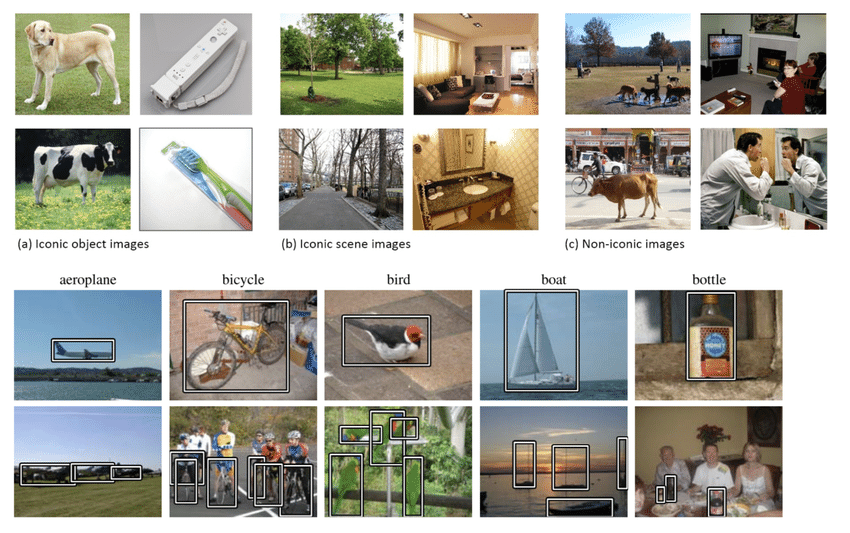
\includegraphics[width=9.5cm]{images/3_1.png}
\caption{Hình 3.1: Hình ảnh trích từ tập dữ liệu COCO}
\end{figure}

\subsection{Chuẩn hoá dữ liệu}\label{normalization}
\noindent
Khi sử dụng Pytorch để xử lí hình ảnh nhờ vào thư viện \texttt{PIL} và \texttt{skimage}, thì khoảng giá trị của không gian màu xám khi đưa về Tensor sẽ là $[0, 1]$, còn không gian màu Lab sẽ là:

\begin{itemize}
    \item \textbf{L} $\in [0, 100]$
    
    \item \textbf{a} $\in [-86.1830, 98.2331]$
    
    \item \textbf{b} $\in [-107.8573, 94.4781]$
\end{itemize}

\noindent
Ta có thể kiểm tra chuyện đó bằng cách:
\begin{lstlisting}
In [2]: import numpy as np
In [3]: colors = np.mgrid[0:256, 0:256, 0:256].astype(np.uint8)
In [4]: colors.shape
Out[4]: (3, 256, 256, 256)

In [6]: all_rgb = np.transpose(colors)
In [7]: from skimage import color
In [8]: all_lab = color.rgb2lab(all_rgb)
In [9]: np.max(all_lab, axis=(0, 1, 2))
Out[9]: array([100.        ,  98.23305386,  94.47812228])

In [10]: np.min(all_lab, axis=(0, 1, 2))
Out[10]: array([   0.        ,  -86.18302974, -107.85730021])
\end{lstlisting}

\noindent
Em quyết định sẽ chuẩn hoá cả đầu vào và đầu ra nằm trong khảong $[-1, 1]$ để áp dụng hàm kích hoạt đầu ra là hàm $\tanh$. Vậy nên, công thức chuẩn hoá sẽ là
\begin{align*}
    \textbf{L}_{\text{normalization}} = \dfrac{\textbf{L}}{50} - 1\\
    \textbf{(a, b)}_{\text{normalization}} = \dfrac{\textbf{(a, b)}}{110}
\end{align*}

\noindent
Bên cạnh đó, kích thước ảnh cũng sẽ được điều chỉnh (\textit{resize}) lại thành ảnh vuông kích thước $256\times 256$.

\subsection{Xây dựng mô hình}

\subsubsection{Generator}
\begin{figure}[h!]
\centering
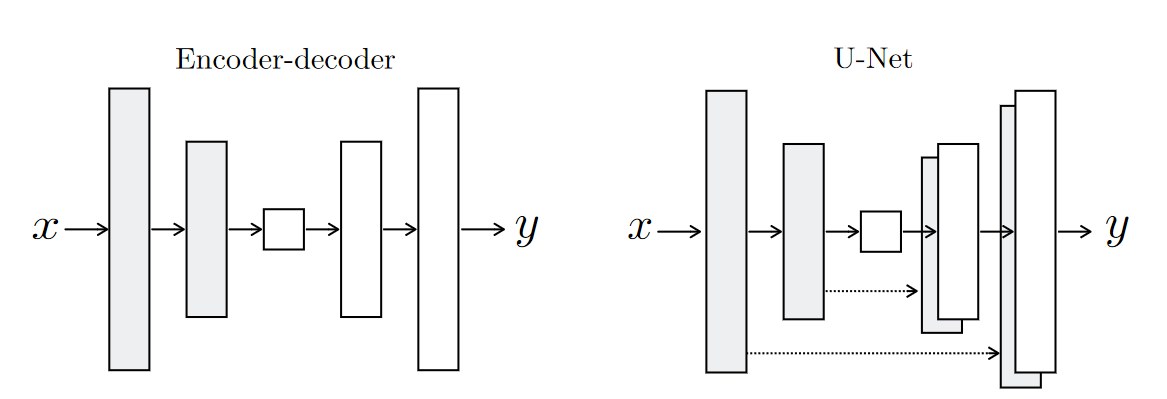
\includegraphics[width=9cm]{images/3_2.PNG}
\caption{Hình 3.2: Một trong 2 lựa chọn cho Generator. Mô hình Encoder-Decoder trái, Unet phải}
\end{figure}

\noindent
Mô hình Generator sẽ nhận đầu vào là một ảnh xám kích thước $256\times 256$, tức là một Tensor có số chiều là $(N, 1, 256, 256)$ với $N$ là batch size, $1$ là $1$ kênh xám. Đầu ra của Generator là một Tensor có số chiều là $(N, 2, 256, 256)$ với $2$ kênh màu \textbf{(a, b)}.\\

\noindent
Giả sử \texttt{Ck} là khối Convolution-BatchNorm-ReLU với $k$ \textbf{bộ lọc} (\textit{kernel/filter}). \texttt{CDk} là khối Convolution-BatchNorm-Dropout-ReLU với tỉ lệ dropout là $50\%$ và $k$ bộ lọc. Tất cả đều sử dụng bộ lọc kích thước $4\times 4$ với \textbf{sải bước} (\textit{stride}) là $2$ và \textbf{đệm} (\textit{padding}) là $1$.\\
Sau mỗi khối \texttt{Ck} sẽ là một khối \textbf{gộp cực đại} (\textit{max-pooling}) để giảm kích thước (không tính chiều sâu) dữ liệu xuống gấp đôi. Còn sau mỗi khối \texttt{CDk} sẽ là một khối \textbf{giải chập} (\textit{deconvolution/upsampling}) thì kích thước dữ liệu tăng gấp đôi.\\
Cụ thể, mô hình sẽ có kiến trúc như chi tiết như sau:

\begin{itemize}
    \item \textbf{encoder:} \texttt{C64-C128-C256-C512-C512-C512-C512-C512}
    
    \item \textbf{decoder:} \texttt{CD512-CD1024-CD1024-C1024-C512-C256-C128}
\end{itemize}

\noindent
Ở \textbf{encoder}, ta sẽ sử dụng hàm LeakyReLU với độ dốc âm là $0.2$ thay vì ReLU. Tầng cuối cùng của Generator sẽ là một hàm $\tanh$. Một ngoại lệ là ở tầng đầu tiên ở \textbf{encoder} ta sẽ không sử dụng BatchNorm.

\subsubsection{$70\times 70$ Patch Discriminator}
Sau khi qua các khối tích chập:

\begin{itemize}
    \item \texttt{C64-C128-C256-C512}
\end{itemize}

\noindent
Một lưu ý ở đây là ở tầng cuối cùng thì sải bước là 1. Ta sẽ đưa qua thêm 1 tầng tích chập với chỉ một bộ lọc để đưa về một Tensor dạng $(N, 1, 30, 30)$ vởi sải bước cũng là 1. Khi này, mỗi vị trí đầu ra sẽ là kết quả xát suất đánh giá xem vùng $70 \times 70$ của đầu vào có thật hay không.\\
Vùng kích thước $70\times 70$ còn được gọi là vùng nhận thức (\textit{receptive field}), đây chính là vùng mà ta sử dụng bộ lọc áp dụng phép toán tính chập để có kết quả là một số.\\

\noindent
Từ đó, để tính kích thước vùng nhận thức ở tầng thứ $l$ bất kì thì ta sẽ có công thức:
\begin{align*}
    K_{l-1} = K + s{l-1}(K_{l} - 1)
\end{align*}
Trong đó $K_l$ là kích thước vùng nhận thức ở tầng thứ $l$, $K$ là kích thước bộ lọc và $s_{l}$ chính là số sải bước ở tầng thứ $l$.

\begin{figure}[h!]
\centering
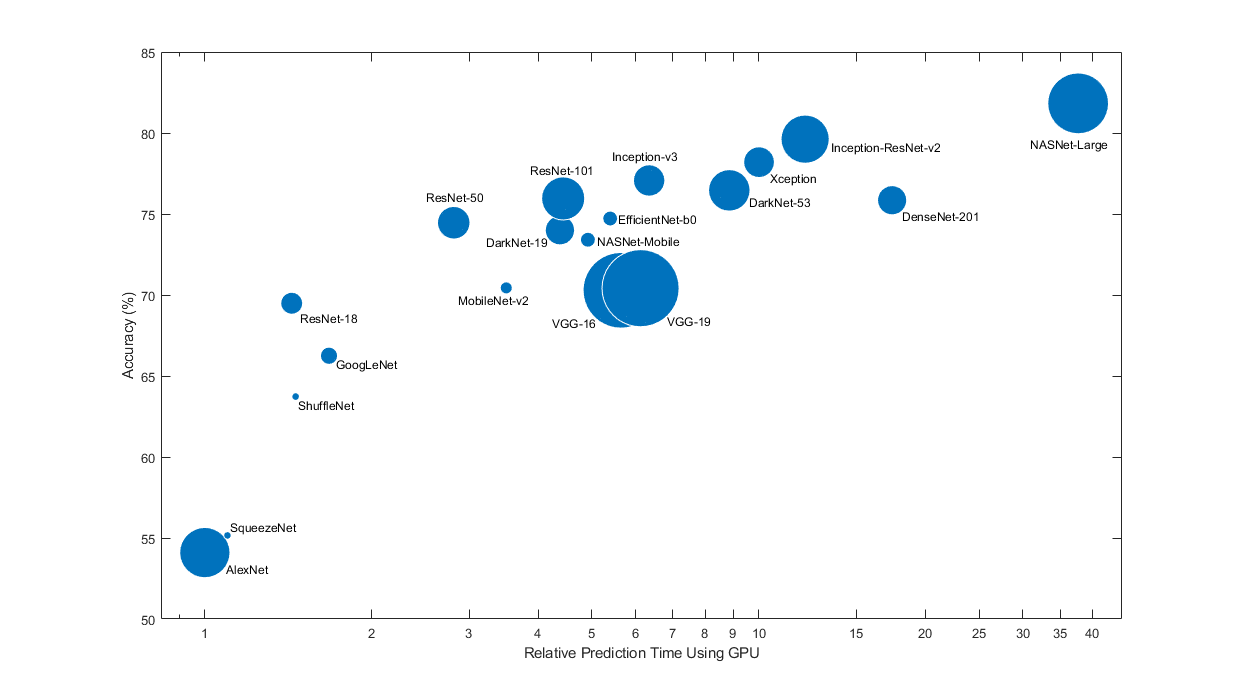
\includegraphics[width=6cm]{images/3_3.png}
\caption{Hình 3.3: Mô tả vùng nhận thức qua các tầng. Nguồn: \href{https://bit.ly/3xGaeLa}{https://bit.ly/3xGaeLa}}
\end{figure}

\noindent
Như vậy, với mỗi đầu ra $1 \times 1$ của kết quả $30\times 30$ thì kích thước vùng nhận thức quét được có thể được tính như sau:
\begin{align*}
    K_4 &= K + s_4(K_5 - 1) = 4 + 1(1-1) = 4\\
    K_3 &= K + s_3(K_4 - 1) = 4 + 1(4-1) = 7\\
    K_2 &= K + s_2(K_3 - 1) = 4 + 2(7-1) = 16\\
    K_1 &= K + s_1(K_2 - 1) = 4 + 2(16-1) = 34\\
    K_0 &= K + s_0(K_1 - 1) = 4 + 2(34 - 1) = 70
\end{align*}


\subsubsection{Sử dụng học chuyển đổi (Transfer learning)}
Sau khi huấn luyện mô hình và thử nghiệm thì thấy kết quả không được khả quan cho lắm. Do đó, em đã quyết định sử dụng một mạng đã được huấn luyện sẵn, tốt để làm nòng cốt, tận dụng các bộ lọc có sẵn cho mô hình Generator. Cụ thể, em sử dụng mạng \textbf{RestNet18}, lí do chọn mạng này là do đây là một mạng phân loại (classification model) có kết quả khá chính xác khi được huấn luyện trên tập dữ liệu \href{http://www.image-net.org/download}{ImageNet}, bên cạnh đó kích thước mô hình này cũng không quá lớn, dễ dàng để huấn luyện hơn.

\begin{figure}[h!]
\centering
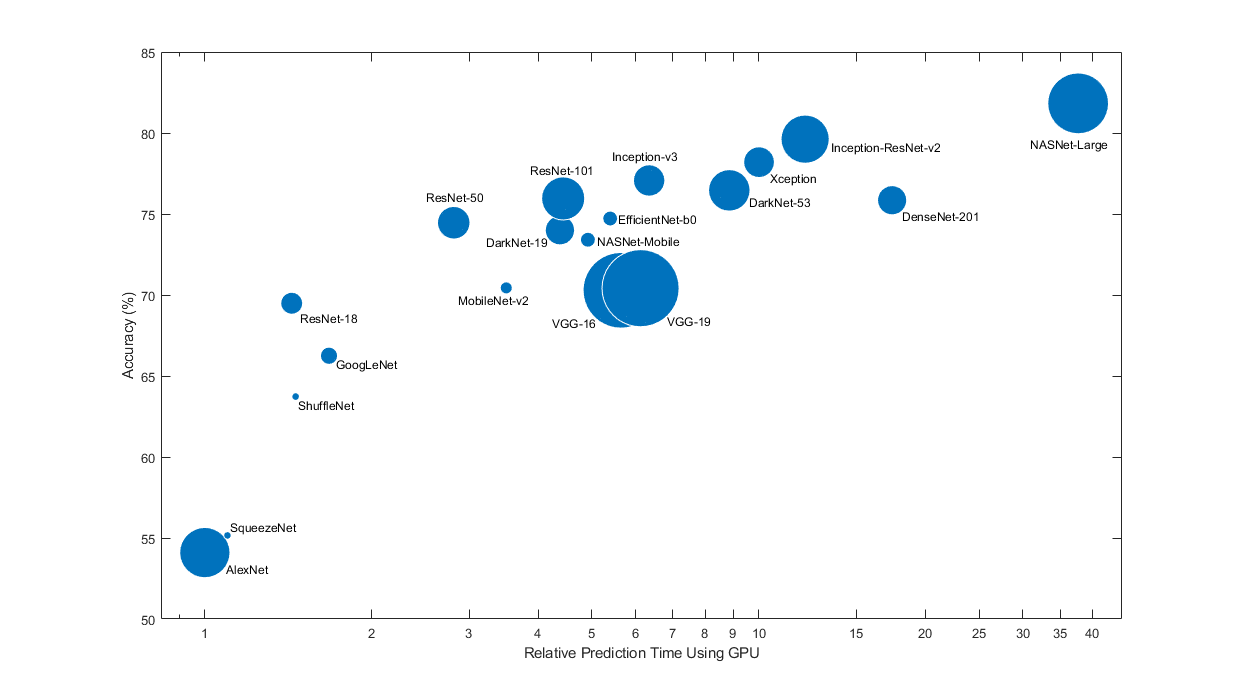
\includegraphics[width=14.4cm]{images/3_4.png}
\caption{Hình 3.4: So sánh các mô hình mạng tích chập hiện đại hiện nay}
\end{figure}

\noindent
Ta có thể dễ dàng xây dựng được một Generator theo kiến trúc mạng Unet dựa vào thông số mạng ResNet18 thông qua thư viện \texttt{fastai}.
\begin{lstlisting}
from fastai.vision.learner import create_body
from fastai.vision.models.unet import DynamicUnet

body = create_body(resnet18, pretrained=True, n_in=1, cut=-2)
G = DynamicUnet(body, 2, (256, 256))
\end{lstlisting}

\subsubsection{Huấn luyện riêng mạng Generator}
Khi huấn luyện GAN, việc khó nhất là huấn luyện cho Generator. Để tối ưu việc đó, ta sẽ đưa riêng ra huấn luyện mạng Generator trước khi đưa vào GAN nhờ vào hàm mất mát $\mathcal{L}_{\text{L1}}(G)$.\\

\noindent
Việc huấn luyện, em sử dụng thuật toán tối ưu Adam với tốc độ học $\alpha =  10^{-4}$, hệ số phân rã (\textit{exponential decay rates}) $\beta_1 = 0.9, \beta_2 = 0.999$ và $\epsilon = 10^{-8}$. Cho chạy batch size là 16 và 30 epoch. Mỗi epoch mất khoảng 6-7 phút (chưa tính phần xác thực).

\begin{figure}[h!]
\centering
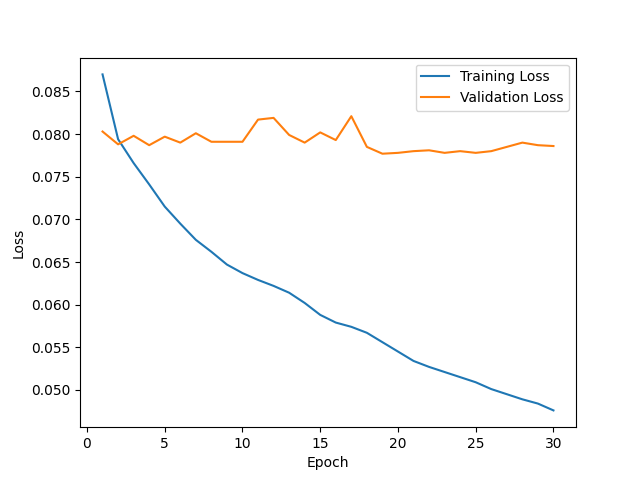
\includegraphics[width=15cm]{images/3_5.png}
\caption{Hình 3.5: Giá trị mất mát của hai tập huấn luyện \& xác thực qua từng epoch}
\end{figure}

\noindent
Giá trị mất mát của mô hình không cao. Bên cạnh đó, ta thấy rằng giá trị mất mát trên tập huấn luyện có xu hướng giảm và tiếp tục giảm, còn giá trị mất mát trên tập xác thực thì có vẻ đã bão hoà. Để tránh \textbf{quá khớp} (\textit{overfitting}), em sẽ chọn mô hình thứ 20 (tức sau khi huấn luyện qua 20 epoch).

\subsubsection{Huấn luyện mạng GAN}
Tải mạng Generator đã được huấn luyện riêng trước đó, sau đó đưa vào để huấn luyện chung với mạng GAN với hệ số cân bằng $\lambda = 100$. Thuật toán tối ưu vẫn sẽ dùng là Adam cho cả hai mạng Generator và Discriminator với các thông số được chọn là:
\begin{align*}
\alpha = 2\times 10^{-4}, \beta = (0.5, 0.999), \epsilon = 10^{-8}
\end{align*}
Cho chạy với batch size là 16 và 20 epoch. Mỗi epoch mất khoảng 10-16 phút (chưa tính phần xác thực).

\begin{figure}[h!]
\centering
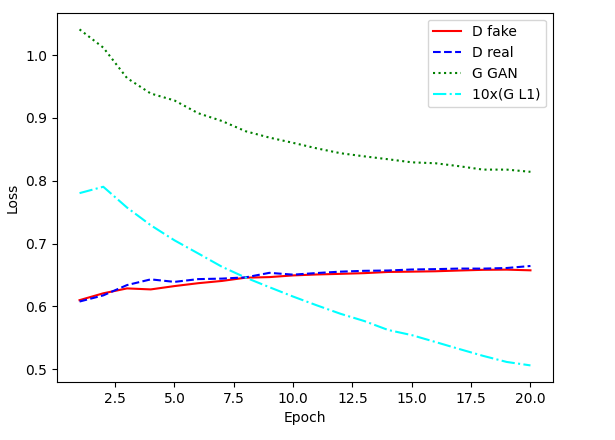
\includegraphics[width=15cm]{images/3_6.png}
\caption{Hình 3.6: Giá trị mất mát của Discriminator và Generator qua từng epoch}
\end{figure}

\noindent
Nhận thấy xu hướng của giá trị mất mát khi huấn luyện mô hình GAN là giá trị mất mát của D tăng thì giá trị mất mát của G sẽ giảm và cả hai đều sẽ hội tụ về một giá trị. Điều này là hợp lí với nguyên lí \textbf{non-zero-sum-games}. Ngoài ra, giá trị mất mát của Generator theo chuẩn 1 cũng được giảm, tuy không nhiều.\\

\noindent
Sau khi xem xét một vài kết quả của mô hình sau mỗi epoch, em quyết định chọn mô hình thứ 15 (tức sau khi huấn luyện qua 15 epoch).

%%%%%%%%%%%%%%%%%%%%%%%%%%%%%%%%%
\section{Thử nghiệm mô hình}

\subsection{Kết quả thực nghiệm của mô hình GAN kết hợp chuẩn 1}\label{experiment}

\begin{figure}[h!]
\centering
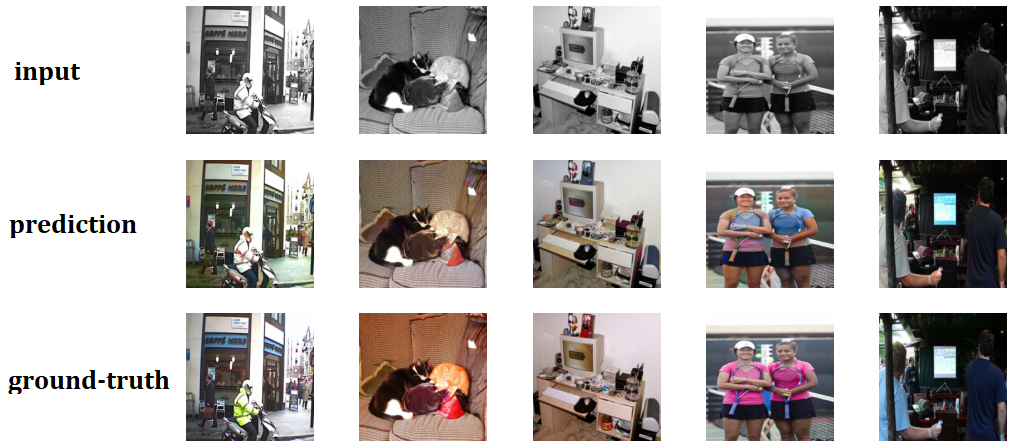
\includegraphics[width=14.4cm]{images/4_1.png}
\caption{Hình 4.1: Kết quả dự đoán của mô hình trên dữ liệu xác thực của tập dữ liệu \textbf{COCO}}
\end{figure}

\noindent
Đây là mô hình được huấn luyện dựa  vào mạng Generator đã được tiền huấn luyện trước với 20 epoch, sau đó kết hợp với huấn luyện đối nghịch với mạng $70\times 70$ Patch Discriminator sau 15 epoch trên tập dữ liệu $10,000$ bức ảnh của \textbf{COCO}.\\
Kết quả cho thấy rằng mô hình sau khi huấn luyện đã có khả năng tô màu cho các đối tượng trong ảnh, màu ít hoặc gần như không bị lem. Mô hình cũng không dự đoán chính xác tuyệt đối màu của một số đối tượng nhưng hợp lí, theo đúng hướng giải quyết vấn đề mà ta mong muốn.\\
Một vài vùng ảnh, mô hình có vẻ như vẫn chưa thực sự tô được màu khi để màu gần giống với mức xám ban đầu. Để lí giải cho hạn chế này, có thể những vùng chưa được tô màu một cách hợp lí là trong quá trình huấn luyện, mô hình chưa được học qua ảnh có bố cục, đối tượng tương tự. Điều này dẫn đến một hạn chế khác nữa là đối với những ảnh không có bố cục rõ ràng (ảnh logo), mô hình hoàn toàn có thể không có khả năng tô được màu vì không nhận diện đối bối cảnh. Thêm một hạn chế khác là mô hình cũng chưa thực sự biết được những điểm ảnh nào sẽ cùng một đối tượng và cùng màu. Cụ thể như hình ảnh hai cố gái cầm vợt tennis (ảnh thứ 2 từ phía bên phải), phần dưới của áo được tô màu hồng, còn phần trên của áo lại màu xanh. Ở đây, nếu tô cho phần áo màu hồng hay màu xanh thì đều chấp nhận được, nhưng mô hình lại chọn cách tô hai phía của áo, do được chia bởi phần cách tay, bởi hai màu khác nhau.\\
Những hạn chế trên, ta hoàn toàn có thể khắc phục bằng cách cho mô hình được huấn luyện thêm với những tập dữ liệu khác. Một hướng khác, ta có thể sử dụng một mạng được huấn luyện trước tốt hơn \textbf{ResNet18} như \textbf{ResNet50}, \textbf{ResNet101} hoặc \textbf{DenseNet}.

\subsection{So sánh giữa mô hình GAN kết hợp chuẩn 1 và mô hình chỉ dùng chuẩn 1}
Việc so sánh giữa hai mô hình này sẽ cho ta cái nhìn về sự ảnh hưởng của mô hình sau khi được huấn luyện đối nghịch. Cụ thể, em đã chủ động lựa chọn ngẫu nhiên một vài (số lượng 5) tấm ảnh từ Google về ảnh chân dung, phong cảnh, toà nhà cũng như những ảnh có nhiều đối tượng (chi tiết) để thử nghiệm.

\begin{figure}[h!]
\centering
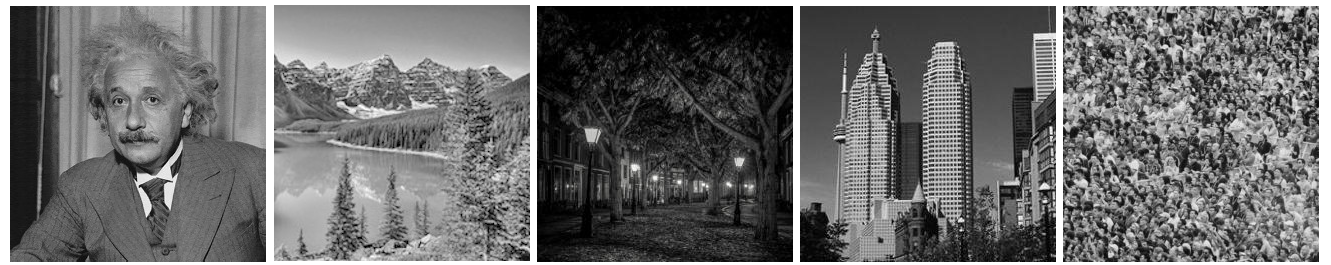
\includegraphics[width=16cm]{images/4_2.PNG}
\caption{Hình 4.2: Những tấm ảnh lựa chọn để thử nghiệm sự khác biệt}
\end{figure}

\noindent
Trước khi đưa cho mô hình dự đoán, không khó để đoán được rằng hình ảnh đầu tiên (phía trái ngoài cùng) có ít chi tiết nhất nên sẽ có kết quả tốt nhất. Ngược lại, hình ảnh cuối cùng (phía phải ngoài cùng) có rất nhiều chi tiết nên kết quả khó có thể đạt được tốt như những tấm ảnh ít chi tiết.\\
Không ngoài dự đoán, kết quả có được khá đúng với những gì mong đợi.

\begin{figure}[h!]
\centering
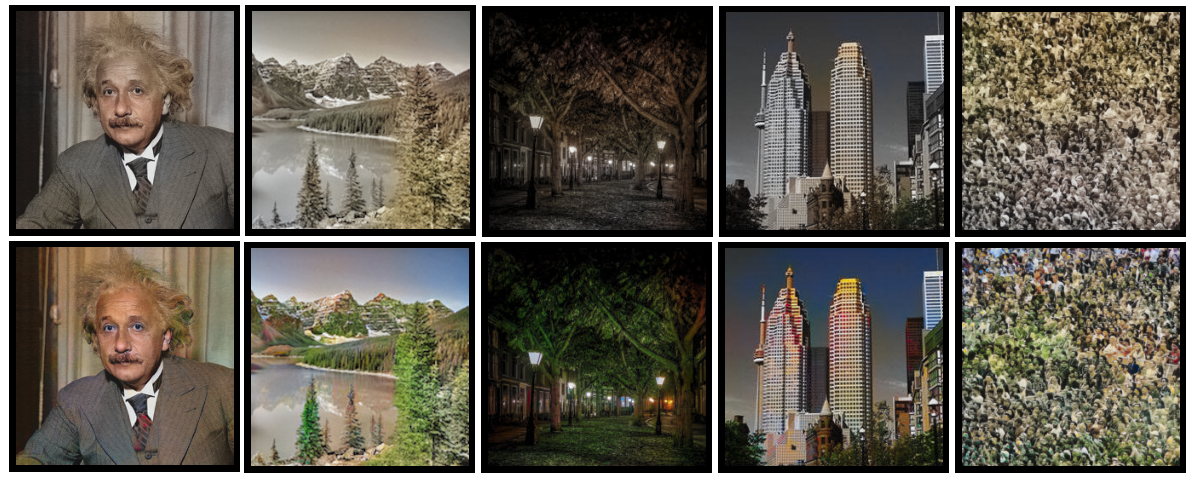
\includegraphics[width=16cm]{images/4_3.PNG}
\caption{Hình 4.3: So sánh kết quả dự đoán của hai mô hình là mô hình chỉ dùng chuẩn 1 (phía trên) với mô hình GAN kết hợp chuẩn 1 (phía dưới)}
\end{figure}

\noindent
Không khó để ta có thể thấy mô hình có sự kết hợp của GAN cho kết quả có màu tươi sáng, chân thật hơn so với khi ta chỉ dùng chuẩn 1. Điều này là do mô hình dùng chuẩn 1 nếu không tìm được màu phù hợp thì sẽ sử dụng giá trị trung bình, tức là giá trị \textbf{(a, b)} $\approx (0, 0)$ vì $-1 \le$ \textbf{a}, \textbf{b} $\le 1$. Khi đó, màu của điểm ảnh sẽ không khác so với mức xám \textbf{L} đầu vào là bao, khiến cho kết quả của mô hình chỉ dùng chuẩn 1 dường nhỉ chỉ là thay đổi độ sáng của ảnh đầu vào chứ không thực sự tô được màu. Và hạn chế này đã được khắc phục rất nhiều khi ta đưa mô hình huấn luyện đối nghịch.

%%%%%%%%%%%%%%%%%%%%%%%%%%%%%%%%%
\section{Kết luận \& Hướng phát triển}

\subsection{Kết luận}
Về kết quả đề tài, mô hình được xây dựng theo kiểu mạng đối nghịch tạo sinh với Generator có kiến trúc Unet dựa theo mạng huấn luyện sẵn ResNet18, sau khi học đã có khả năng tự động tô màu những ảnh xám, cũ một cách chân thực, hợp lí. Dẫu vậy, mô hình vẫn chưa có kết quả tốt khi áp dụng với những ảnh có bố cục, đối tượng mà mô hình chưa được học trong quá trình huấn luyện. Tuy vậy, như đã đề cập ở phần \textbf{4.1 \nameref{experiment}}, ta hoàn toàn có thể cải thiện trí tuệ mô hình thông qua việc tìm thêm nhiều tập dữ liệu với các bố cục, đối tượng phong phú để huấn luyện thêm.\\
So với mục tiêu đề ra trong phần \textbf{1.2 \nameref{objective}}, khi xây dựng một mô hình dự đoán được màu của những đối tượng trong ảnh xám một cách hợp lí, chất lượng không yêu cầu phải tốt như làm thủ công, giúp tiết kiệm thời gian trong quá trình phục hồi màu cho ảnh xám thì mô hình đã xử lí được vấn đề được nêu ra.\\

\noindent
Sau quá trình tìm hiểu và hoàn thành đề tài, bản thân em đã học thêm được nhiều kiến thức về những không gian màu của ảnh số ngày nay (RGB, Lab). Thêm vào đó, nhờ việc thực sự đắm mình vào học sâu (\textit{dive into deep learning}), em đã có một cái nhìn rõ ràng hơn về học máy/học sâu trong một mảng khổng lồ như là \textbf{trí tuệ nhân tạo} (\textit{artificial intelligence}).

\subsection{Hướng phát triển}
Đề tài có thể được áp dụng để làm những tác vụ liên quan đến phục chế màu cho ảnh xám, bị mất màu. Giúp cho quá trình phục chế được tiết kiệm thời gian. Kết hợp với tinh chỉnh bằng phương pháp thủ công, ta hoàn toàn có thể có những kết quả phục chế đẹp đẽ và cũng nhanh chóng.\\
Không chỉ dừng lại ở hình ảnh, ta cũng có thể áp dụng mô hình để phục chế màu cho video, khi cắt từng khung (\textit{frame}) hình ra phục chế sau đó ghép lại.

\begin{figure}[h!]
\centering
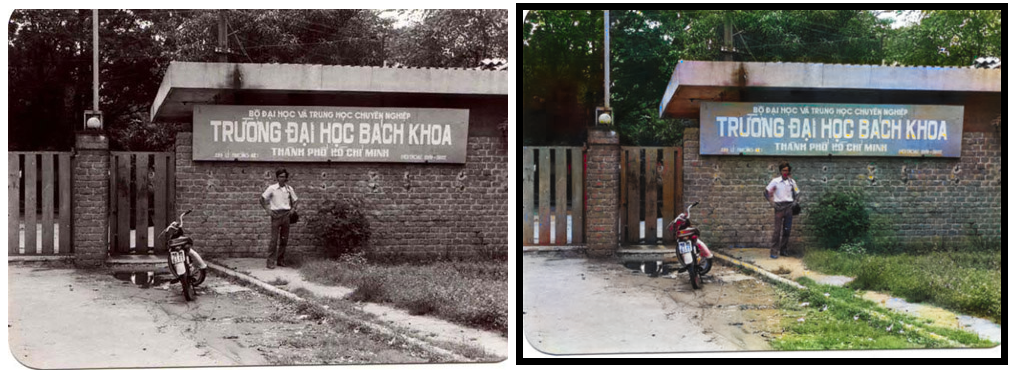
\includegraphics[width=17cm]{images/5_1.PNG}
\caption{Hình 5.1: Ảnh Trường ĐH Bách Khoa TP.HCM ngày xưa (trái) và sau khi tô màu (phải)}
\end{figure}

\clearpage

%%%%%%%%%%%%%%%%%%%%%%%%%%%%%%%%%
\section{Phục lục - Ảnh màu}
\begin{figure}[h!]
\centering
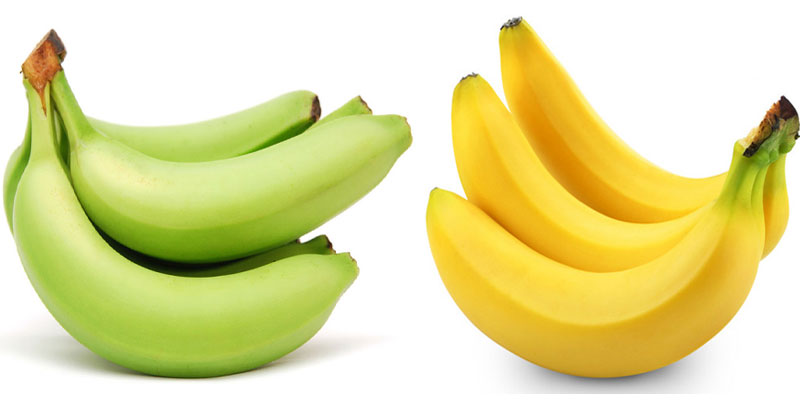
\includegraphics[width=15cm]{images/1_1.jpg}
\caption*{Hình 1.1: Nải chuối có thể màu lục hoặc màu vàng. Nguồn: \href{https://bit.ly/3e7nqRs}{https://bit.ly/3e7nqRs}}
\end{figure}

\begin{figure}[h!]
\centering
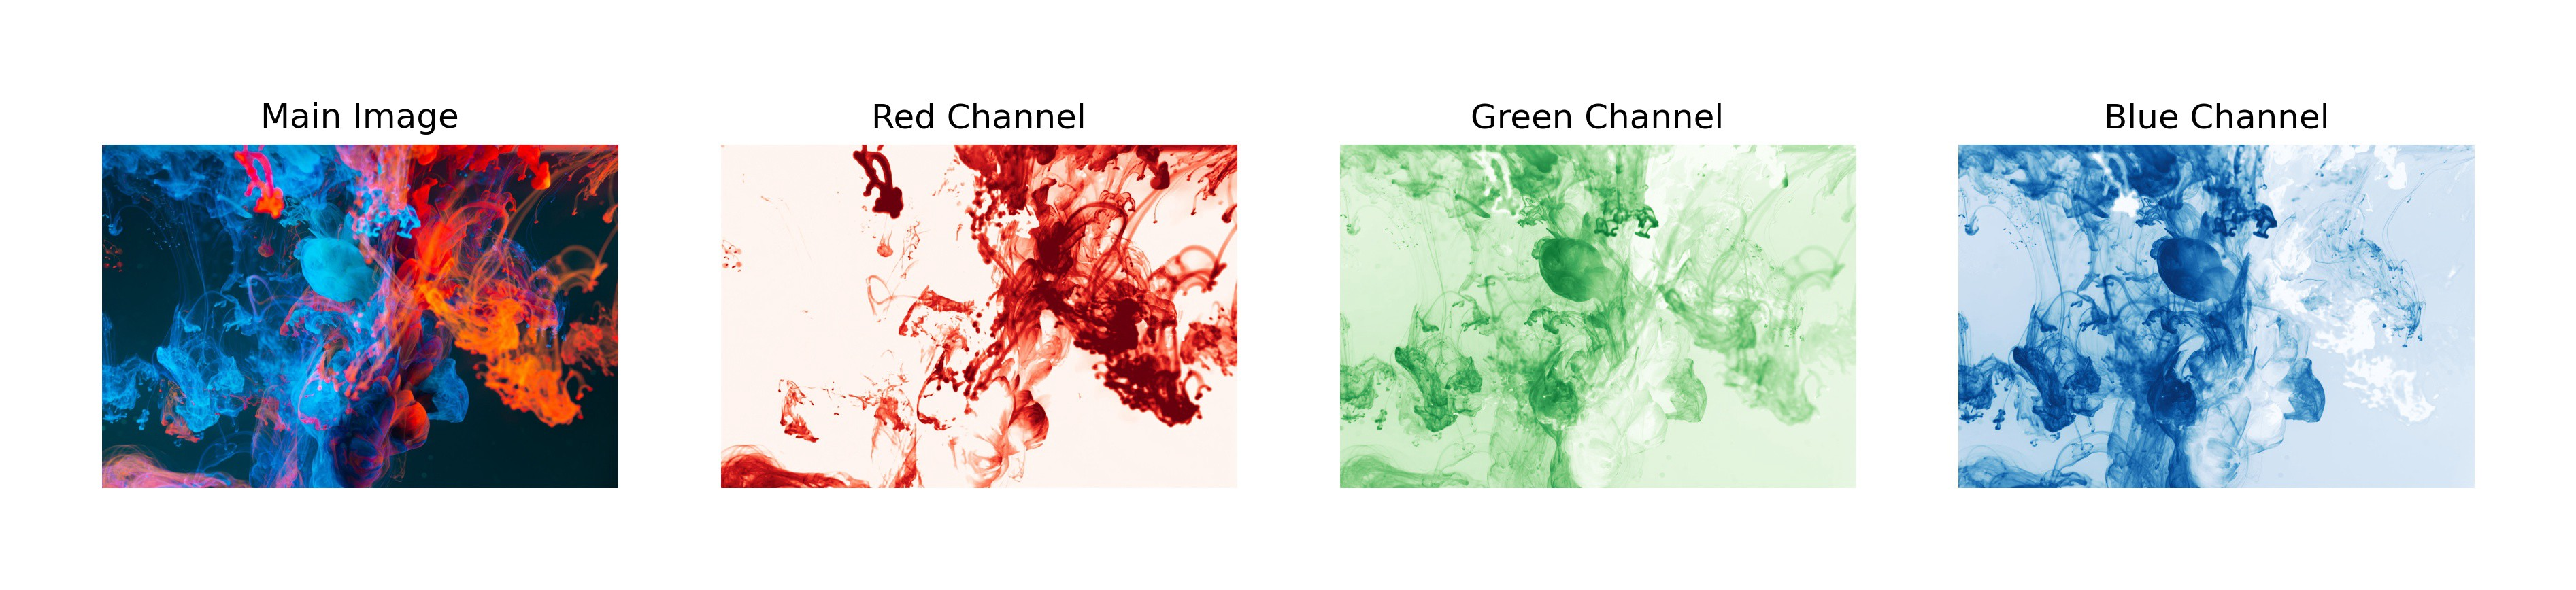
\includegraphics[width=16.1cm]{images/2_1.jpeg}
\caption*{Hình 2.1: Các kênh màu đỏ, lục và lam được tách ra riêng biệt. Nguồn: \href{https://bit.ly/3eKaaBj}{https://bit.ly/3eKaaBj}}
\end{figure}

\begin{figure}[h!]
\centering
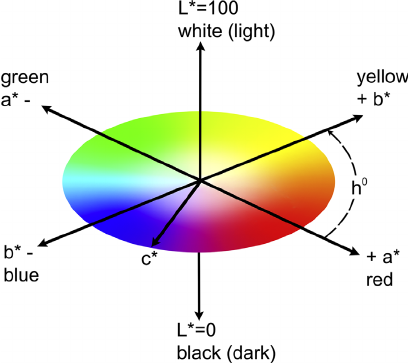
\includegraphics[width=5.8cm]{images/2_2.png}
\caption*{Hình 2.2: Không gian màu Lab. Nguồn: \href{https://bit.ly/3nFIQIp}{https://bit.ly/3nFIQIp}}
\end{figure}

\begin{figure}[h!]
\centering
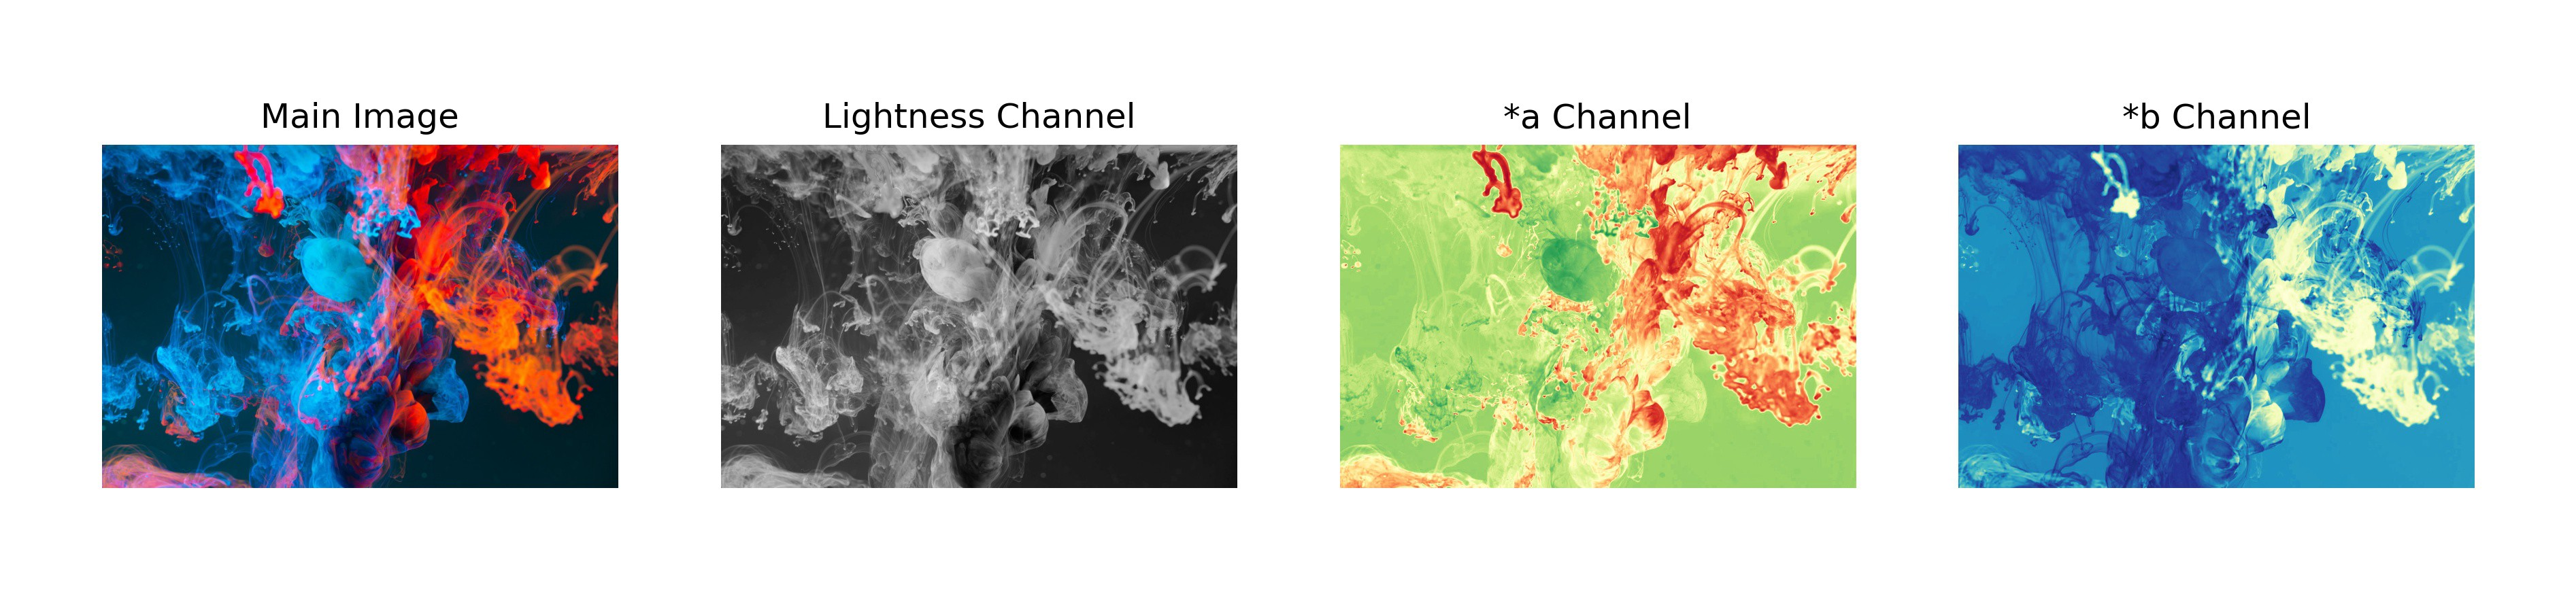
\includegraphics[width=16.1cm]{images/2_3.jpeg}
\caption*{Hình 2.3: Các giá trị \textbf{L}, \textbf{a} và \textbf{b} được tách ra riêng biệt. Nguồn: \href{https://bit.ly/3eKaaBj}{https://bit.ly/3eKaaBj}}
\end{figure}

\begin{figure}[h!]
\centering
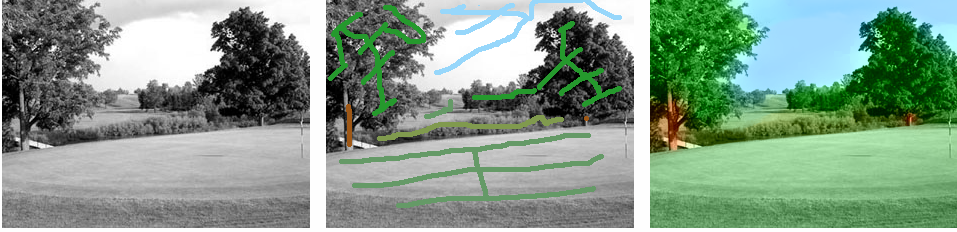
\includegraphics[width=15cm]{images/2_4.png}
\caption*{Hình 2.4: Mô tả ý tưởng thuật toán. Nguồn: \href{https://bit.ly/3eKdmwN}{https://bit.ly/3eKdmwN}}
\end{figure}

\begin{figure}[h!]
\centering
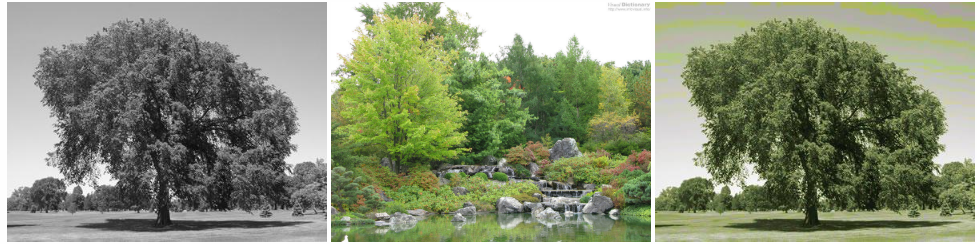
\includegraphics[width=15cm]{images/2_5.png}
\caption*{Hình 2.5: Mô tả ý tưởng thuật toán. Nguồn: \href{https://bit.ly/3eKdmwN}{https://bit.ly/3eKdmwN}}
\end{figure}

\begin{figure}[h!]
\centering
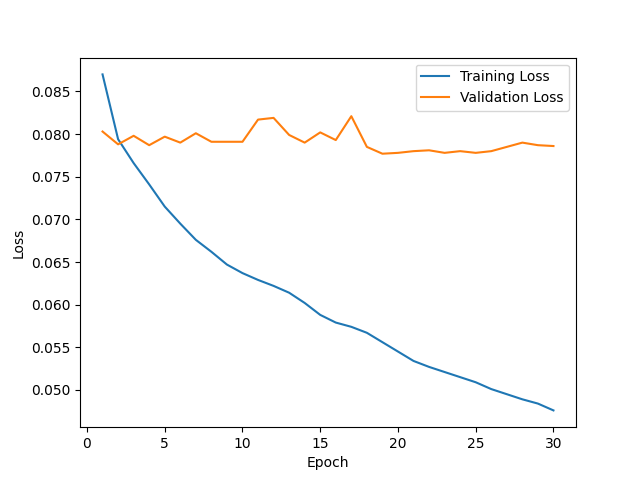
\includegraphics[width=15cm]{images/3_5.png}
\caption*{Hình 3.5: Giá trị mất mát của hai tập huấn luyện \& xác thực qua từng epoch}
\end{figure}

\begin{figure}[h!]
\centering
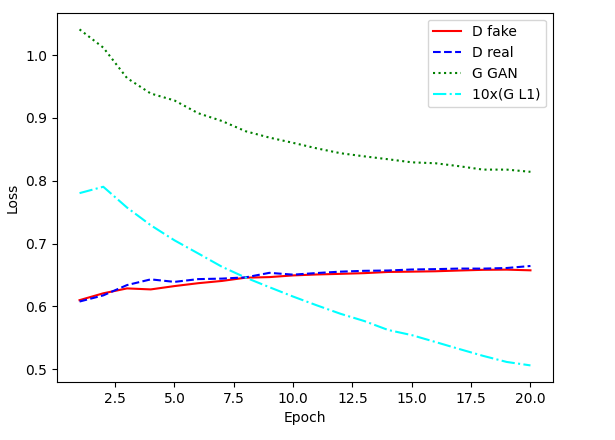
\includegraphics[width=15cm]{images/3_6.png}
\caption*{Hình 3.6: Giá trị mất mát của Discriminator và Generator qua từng epoch}
\end{figure}

\begin{figure}[h!]
\centering
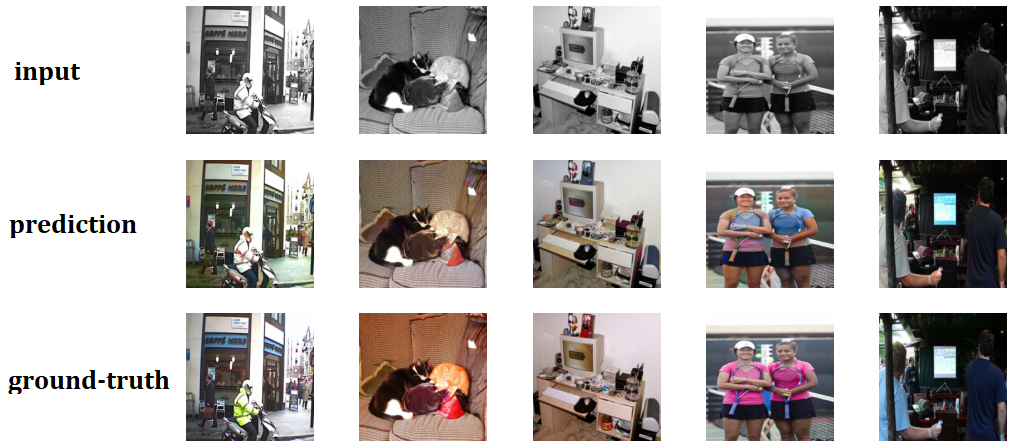
\includegraphics[width=14.4cm]{images/4_1.png}
\caption*{Hình 4.1: Kết quả dự đoán của mô hình trên dữ liệu xác thực của tập dữ liệu \textbf{COCO}}
\end{figure}

\begin{figure}[h!]
\centering
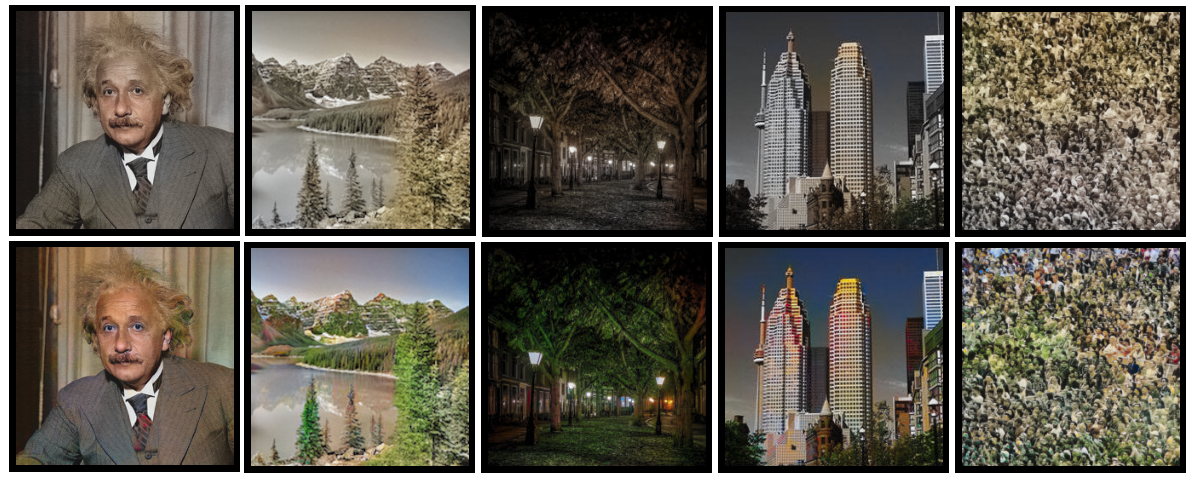
\includegraphics[width=16cm]{images/4_3.PNG}
\caption*{Hình 4.3: So sánh kết quả dự đoán của hai mô hình là mô hình chỉ dùng chuẩn 1 (phía trên) với mô hình GAN kết hợp chuẩn 1 (phía dưới)}
\end{figure}

\begin{figure}[h!]
\centering
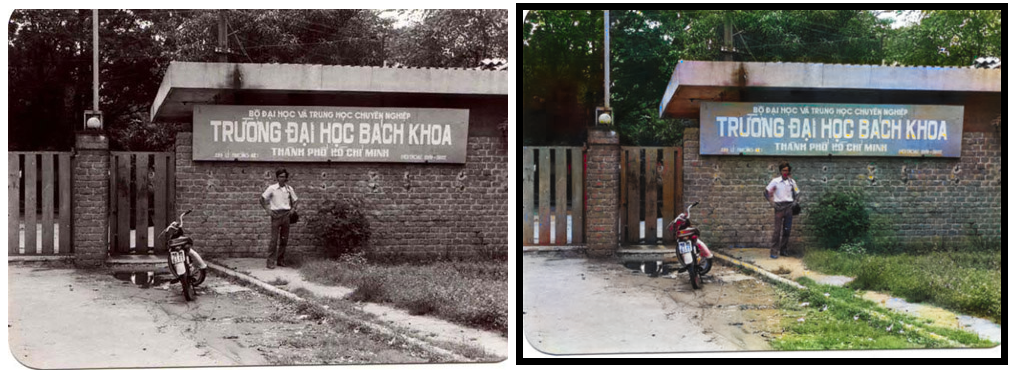
\includegraphics[width=17cm]{images/5_1.PNG}
\caption*{Hình 5.1: Ảnh Trường ĐH Bách Khoa TP.HCM ngày xưa (trái) và sau khi tô màu (phải)}
\end{figure}

\clearpage

\renewcommand{\refname}{Tài liệu tham khảo}
%%%%%%%%%%%%%%%%%%%%%%%%%%%%%%%%%
\begin{thebibliography}{80}\label{references}

    \bibitem{aladdinpersson} Aladdin Persson, Building our first simple GAN, \href{https://youtu.be/OljTVUVzPpM}{https://youtu.be/OljTVUVzPpM}, (2020).

    \bibitem{aladdinpersson} Aladdin Persson, Pix2Pix Paper Walkthrough, \href{https://youtu.be/SuddDSqGRzg}{https://youtu.be/SuddDSqGRzg}, (2021).

    \bibitem{aladdinpersson} Aladdin Persson, Pix2Pix implementation from scratch, \href{https://youtu.be/SuddDSqGRzg}{https://youtu.be/SuddDSqGRzg}, (2021).

    \bibitem{aladdinpersson} Aladdin Persson, U-NET Paper Walkthrough, \href{https://youtu.be/oLvmLJkmXuc}{https://youtu.be/oLvmLJkmXuc}, (2021).

    \bibitem{connorshorten} Connor Shorten, DCGANs (Deep Convolutional Generative Adversarial Networks),\\ \href{https://bit.ly/3nFC7OC}{https://bit.ly/3nFC7OC}, (2018).

    \bibitem{cornorshorten} Cornor Shorten, Pix2Pix, \href{https://bit.ly/3eMDGGt}{https://bit.ly/3eMDGGt}, (2019).

    \bibitem{elistevens} Eli Stevens, Luca Antiga, Thomas Viehmann and Foreword by Soumith Chintala, Deep Learning with PyTorch, Manning Publications, New York (2020).

    \bibitem{emilwallner} Emil Wallner, How to colorize black \& white photos with just 100 lines of neural network code, \href{https://bit.ly/3u8uSkN}{https://bit.ly/3u8uSkN}, (2017).

    \bibitem{harshalllamba} Harshall Lamba, Understanding Semantic Segmentation with UNET, \href{https://bit.ly/3tdDK7B}{https://bit.ly/3tdDK7B}, (2019).

    \bibitem{goodfellow} Ian J. Goodfellow et al. Generative Adversarial Networks, \href{https://arxiv.org/abs/1406.2661}{https://arxiv.org/abs/1406.2661}, (2014).

    \bibitem{jasonbrownlee} Jason Brownlee, A Gentle Introduction to Pix2Pix Generative Adversarial Network,\\ \href{https://bit.ly/2RhbbsC}{https://bit.ly/2RhbbsC}, (2019).

    \bibitem{josephrocca} Joseph Rocca, Understanding Generative Adversarial Networks (GANs), \href{https://bit.ly/3vzdPIU}{https://bit.ly/3vzdPIU}, (2019).

    \bibitem{juan} Juan, What range does skimage use in LAB color space for each channel?, \href{https://bit.ly/3eaonbt}{https://bit.ly/3eaonbt}, (2020).

    \bibitem{mehdimirza} Mehdi Mirza \& Simon Osindero, Conditional Generative Adversarial Nets,\\ \href{https://arxiv.org/abs/1411.1784}{https://arxiv.org/abs/1411.1784}, (2014).

    \bibitem{moeinshariatnia} Moein Shariatnia, Colorizing black \& white images with U-Net and conditional GAN — A Tutorial, \href{https://bit.ly/3eKaaBj}{https://bit.ly/3eKaaBj}, (2020).

    \bibitem{olafronneberger} Olaf Ronneberger, Philipp Fischer \& Thomas Brox, U-Net: Convolutional Networks for Biomedical Image Segmentation, \href{https://arxiv.org/abs/1505.04597}{https://arxiv.org/abs/1505.04597}, (2015)

    \bibitem{phamdinhkhanh} Pham Dinh Khanh, Image Segmentation, \href{https://bit.ly/335IEZE}{https://bit.ly/335IEZE}, (2020).

    \bibitem{phillipisola} Phillip Isola, Jun-Yan Zhu, Tinghui Zhou \& Alexei A. Efros, Image-to-Image Translation with Conditional Adversarial Networks, \href{https://arxiv.org/abs/1611.07004}{https://arxiv.org/abs/1611.07004}, (2016).

    \bibitem{richardzhang} Richard Zhang, Phillip Isola \& Alexei A. Efros, Colorful Image Colorization,\\ \href{https://arxiv.org/abs/1603.08511}{https://arxiv.org/abs/1603.08511}, (2016).

    \bibitem{sahil} Sahil, Understanding PatchGAN, \href{https://bit.ly/3xJy0Wo}{https://bit.ly/3xJy0Wo}, (2020).

    \bibitem{trungthanhnguyen} Trung Thanh Nguyen, Auto Colorize Grayed Image With Deep Learning, \href{https://bit.ly/3theTj4}{https://bit.ly/3theTj4}, (2018).

    \bibitem{tuannguyen} Tuan Nguyen, Conditional GAN (cGAN), \href{https://bit.ly/3udFFKH}{https://bit.ly/3udFFKH}, (2020).

    \bibitem{tuannguyen} Tuan Nguyen, Deep Convolutional GAN (DCGAN), \href{https://bit.ly/3uhxtcb}{https://bit.ly/3uhxtcb}, (2020).

    \bibitem{tuannguyen} Tuan Nguyen, Giới thiệu về GAN, \href{https://bit.ly/3aXhHvD}{https://bit.ly/3aXhHvD}, (2019).

    \bibitem{tuannguyen} Tuan Nguyen, Pix2pix, \href{https://bit.ly/3xGVR9h}{https://bit.ly/3xGVR9h}, (2020).

\end{thebibliography}
\end{document}